%\RequirePackage[swedish]{babel}
%\documentclass[a4paper,reqno,draft,twoside]{amsbook}
\documentclass[a4paper,reqno,final,twoside]{amsbook}
\usepackage{fixltx2e}
\usepackage[latin1]{inputenc}
\usepackage[T1]{fontenc}
\usepackage{graphicx}
\usepackage{url}
\usepackage{hyperref}
\usepackage{lettrine}
\usepackage[german,english,ibycus,swedish]{babel}
\usepackage{amssymb}
\usepackage{amsmath}
\usepackage{amsthm}
%\usepackage[amsmath,hyperref,thmmarks]{ntheorem}
\usepackage{natbib}
\usepackage{setspace}
\usepackage{nomencl}
\usepackage{marginnote}
\usepackage{subfig}
%\usepackage{enumerate}
\usepackage{verbatim}
\usepackage{ifdraft}
\ifdraft{
	\usepackage{fancyhdr}
%	\usepackage{showlabels}
%	\includeonly{intro,logik,mangder,naturliga,heltalen,talsystem}
}{
	\usepackage[a4paper,rmargin=6cm,lmargin=3cm,bmargin=3.5cm]{geometry}
}

\newtheorem{theorem}{Sats}[chapter]
\newtheorem{lemma}[theorem]{Lemma}
\newtheorem{corollary}[theorem]{Korollarium}
\theoremstyle{definition}
\newtheorem{axiom}[theorem]{Axiom}
\newtheorem{definition}[theorem]{Definition}
\newtheorem{example}[theorem]{Exempel}
\newtheorem{exercise}[theorem]{�vning}
\theoremstyle{remark}
\newtheorem{remark}[theorem]{Anm�rkning}
%\newtheorem*{note}[theorem]{Notera}

\numberwithin{section}{chapter}
\numberwithin{equation}{chapter}

\newcommand{\chref}[1]{Kapitel \ref{#1}}
\newcommand{\secref}[1]{avsnitt \ref{#1}}
\newcommand{\appref}[1]{Appendix \ref{#1}}
\newcommand{\tblref}[1]{Tabell \ref{#1}}
\newcommand{\figref}[1]{Figur \ref{#1}}
\newcommand{\axref}[1]{Axiom \ref{#1}}
\newcommand{\defref}[1]{Definition \ref{#1}}
\newcommand{\thmref}[1]{Sats \ref{#1}}
\newcommand{\lemref}[1]{Lemma \ref{#1}}
\newcommand{\corref}[1]{Korollarium \ref{#1}}
\newcommand{\exref}[1]{Exempel \ref{#1}}
\newcommand{\xrcref}[1]{�vning \ref{#1}}

\newcommand{\imp}[1]{\emph{#1}\marginnote{#1}}
%\newcommand{\maybeskip}[1][F�rdjupningsavsnitt.]{\protect\footnote{#1}}
\newcommand{\maybeskip}[1][F�rdjupningsavsnitt.]{\relax}

\renewcommand{\qedsymbol}{Q.E.D.}
\newcommand{\N}{\mathbb{N}}
\newcommand{\Q}{\mathbb{Q}}
\newcommand{\R}{\mathbb{R}}
\newcommand{\Z}{\mathbb{Z}}
\newcommand{\powerset}{\mathcal{P}}
\newcommand{\U}{\mathcal{U}}
\newcommand{\V}{\mathcal{V}}
\DeclareMathOperator{\card}{card}
\DeclareMathOperator{\tnot}{icke}
\DeclareMathOperator{\tor}{eller}
\DeclareMathOperator{\tand}{och}
\newcommand{\equivalent}{\Longleftrightarrow}

\makenomenclature
\makeindex

\begin{document}
\ifdraft{
	\fancypagestyle{plain}{
		\renewcommand{\headrulewidth}{0pt}
		\fancyhead{}
		\fancyfoot[co,ce]{\thepage}
		\fancyfoot[ro,le]{dbosk-\today}
	}
	\fancypagestyle{ams}{
		\renewcommand{\headrulewidth}{0pt}
		\fancyhead[ce]{\small\leftmark}
		\fancyhead[co]{\small\rightmark}
		\fancyhead[lo,re]{}
		\fancyhead[ro,le]{\thepage}
		\fancyfoot[ro,le]{dbosk-\today}
	}
	\pagestyle{ams}
}{}
\title{
	%Mathematica prima gamma\\
	Matematik 1c
}
\date{\today}
\author{Daniel Bosk}
\address{Sandgatan 6, 860\,35 S�r�ker}
\email{\url{dbosk@kth.se}}
\urladdr{\url{http://www.bosk.se/}}
%\thanks{...}

\frontmatter
\begin{abstract}
    \noindent
    ...

\end{abstract}

\ifdraft{}{
    \newgeometry{rmargin=4cm,lmargin=4cm}
}
\maketitle
\ifdraft{}{
    \restoregeometry
}
%\begin{titlepage}
%   \begin{center}
%       \vskip0.1\textheight
%       \textsc{\huge \...@title}
%       \vskip0.1\textheight
%       \textsc{\large \...@author}
%       \vskip0.7\textheight
%       \textsc{\...@date}
%   \end{center}
%\end{titlepage}

\printnomenclature
\tableofcontents

%\chapter*{F�rord}
\noindent
\lettrine{D}{agens matematikundervisning} har f�tt mycket kritik p� sistone,
bland annat i Skolinspektionens rapport 2010:13 \emph{Undervisningen i
matematik i gymnasieskolan}.
Matematiken upplevs som r�knecentrerad och eleverna l�r sig genom memorering
snarare �n f�rst�else.

Detta kompendium syftar till att l�gga grunden f�r en formalisering av
gymnasiematematiken, det �r en b�rjan till undervisningsmaterial utformat
efter �mnesplanen f�r Matematik 1c i Gy2011.
Omfattningen av detta material �r en inledning till rigor�s matematik, en grund
att bygga fortsatt undervisning p�.
Syftet med detta material �r s�ledes inte att vara ett f�rdjupningsmaterial,
utan att formalisera matematiken i dagens gymnasieundervisning.

Materialet �r framtaget med tanken att akompanieras av en undervisande l�rare.

I \appref{app:Kursplanering} till detta kompendium finns en f�reslagen
kursplanering f�r hela kursen Matematik 1c.

De svenska kursplanerna f�r matematik, b�de de gamla och de nya
�mnesplanerna, fokuserar mycket p� till�mpad matematik.
Det g�r �ven de flesta matematikb�cker f�r skolan.
Detta kompendium fokuserar mer p� \emph{ren matematik} eftersom att matematiken
s�llan framh�lls i sin rena form -- kompendiet h�lls dock inom ramarna f�r
�mnesplanen.
Kompendiet �r ocks� upplagt annorlunda och ej avsett att f�lja den
traditionella svenska matematikundervisningen med exempel och m�nga
uppgifter som f�jer exemplet.
Faktum �r att detta kompendium inte inneh�ller en enda s� kallad
standarduppgift.
Det inneh�ller inte n�gra uppgifter i �verhuvudtaget, det inneh�ller �vningar.
Dessa syftar till att l�ta l�saren �va sitt matematiska resonerande.
Hela syftet f�r kompendiet �r faktiskt att f�r�ndra den svenska
matematikundervisningen till att innefatta matematik, riktig matematik, s� som
den b�r upplevas.

Till sist vill jag rikta ett stort tack till mina handledare Roy Skjelnes vid
Kungliga Tekniska H�gskolan, Lil Engstr�m vid Stockholms universitet och
till Dan Laksov f�r v�rdefulla kommentarer och givande diskussioner.


\mainmatter
\ifdraft{
	\doublespacing
}{}
% main chapters
\chapter{Introduktion}
\label{ch:Intro}
\nocite{Kiselman2008mfs}
% TODO f�rb�ttra introduktionen.
% fysik, kemi anv�nder matematiken
\noindent
\lettrine{M}{atematiken har funnits} i mer �n 5000 �r, men b�rjade utvecklas i
riktning mot dagens matematik f�rst omkring 300 f.Kr. i antikens Grekland.
Innan dess var matematiken endast r�kning, ett verktyg f�r att ber�kna skatter
och konstruera byggnadsverk.

Ordet matematik har sitt ursprung i grekiskans \emph{\ibygr{ma'qhma}
(m{\'a}th{\=e}ma)}\nocite{OED} som betyder \emph{l�rande, studier, vetenskap}.
Det �r i det antika Grekland som dagens matematik har sitt ursprung.
De studerade fr�mst geometri och gjorde detta genom att s�tta upp n�gra
grundl�ggande antaganden, kallade postulat eller axiom, som de var �vertygade
om att de st�mde �verens med verkligheten.
Dessa var enkla antaganden, s�som att tv� parallella linjer aldrig kommer att
sk�ra varandra.
Utifr�n dessa enkla postulat h�rledde de olika geometriska resultat och de
kunde bevisa att det m�ste vara p� ett visst s�tt.
�ven om de kunde se genom n�gra enkla experiment hur saker f�rh�ll sig till
varandra n�jde de sig inte utan ett bevis utifr�n postulaten och tidigare
bevisade resultat.

Detta har verkat som inspiration f�r matematiker genom historien och �r den
drivkraft som verkat f�r att matematiken utvecklats till det som den �r idag.
Dagens matematik bygger likt grekernas p� n�gra enkla grundantaganden som vi
kallar f�r axiom.
Vidare m�ste begrepp som vi anv�nder definieras tydligt s� att vi vet exakt vad
som menas med dem.
Detta var drivkraften bakom axiomatiseringen av de naturliga talen som vi
kommer att se i \chref{ch:Naturliga}, bakom grundl�ggningen av de hela talen i
\chref{ch:Heltalen} och de �vriga talen.
L�nge hade matematikerna tagit talen som sj�lvklara, men vid 1800-talets mitt
beh�vde de veta tydligare vad ett tal var f�r att kunna g� vidare.

I en definition av ett objekt eller egenskap s�tter vi upp regler f�r hur ett
objekt som �r av denna typ eller har denna egenskap ska bete sig.
Om vi kan visa att ett objekt uppfyller reglerna i definitionen, d� m�ste
objektet ocks� vara av den typen eller ha den egenskapen.
D� vet vi exakt, vi kan bevisa att ett objekt �r av en specifik typ.
Vi kan ocks� g�ra det omv�nda, om ett objekt �r av denna typen uppfyller det de
givna reglerna.
D� n�r vi bevisar saker kan vi utg� fr�n enbart dessa regler.


%%%%%%%%%%%%%%%%%%%%%%%%%%%%%%%%%%%%%
% VAD �R MATEMATIK?
%%%%%%%%%%%%%%%%%%%%%%%%%%%%%%%%%%%%%
\section{Vad �r d� matematik?}
% - Skillnaden mellan matematiken och andra vetenskaper.
% - Abstrakt konstruktion som endast finns i sinnet.
% - Naturvetenskap i sverige, filosofi i resten av v�rlden.
%   - Sveriges st�rta bidrag till matematikhistorien �r att vi tog d�d p� Ren�
%     Descartes (Touraine, 1596 -- Stockholm, 1650).
% - Beh�ver inte ha n�gon till synes uppenbar till�mpning, det �r vackert.
%   - Pierre de Fermat (160{1,7,8} -- 1665), advokat, upphovsman till Fermats
%     lilla sats och Fermats stora (sista) sats.
%   - Fermat-Euler satsen �r grunden f�r kryptosystemet n�r man loggar in p�
%     banken via Internet.
% - Demokratiskt organiserad. Alla kan bidra, ex. Fermat var advokat.
\noindent
\lettrine{M}{atematiken kan beskrivas} som studiet av abstrakta konstruktioner.
Med abstrakta konstruktioner menar vi saker som endast finns i v�rt sinne.
Vi s�tter upp axiomen och definitionerna, spelreglerna, och unders�ker sedan
vad dessa spelregler ger upphov till.

Historiskt har matematiken ofta varit sammankopplad med studiet av
verkligheten.
Vi har kunnat studera verkligheten med hj�lp av matematiken genom att v�ra
grundregler varit grundl�ggande principer f�r verkligheten\footnote{Se
exempelvis Euklides postulat f�r geometrin.}.
Men trots detta �r matematiken skild fr�n verkligheten.
De axiom vi utg�r ifr�n beh�ver inte vara principer fr�n verkligheten.
Det finns matematiska konstruktioner som kan te sig s� verklighetsfr�nkopplade
att icke-matematiker ifr�gas�tter varf�r de studeras, och detta f�r oss in p�
ett viktigt konstaterande.
%Matematiken har inte alltid studerats enbart f�r att kunna dra slutsatser om
%verkligheten.
M�nga matematiker genom historien studerade matematiken enbart f�r den rena
matematikens skull -- f�r att den var vacker, inte f�r att den gick att
till�mpa p� verkligheten.
%F�r att utforska den v�rld som sp�nns upp av axiomen.
Exempel p� s�dana �r Pierre de Fermat (ca 1607-1650) som �r upphovsman till den
k�nda \emph{Fermats stora sats}.
Han var advokat och amat�rmatematiker.
\emph{Fermats stora sats} eller \emph{Fermats sista sats} s�ger att ekvationen
\(x^n+y^n=z^n\), d�r \(x,y\) och \(z\) �r heltal, saknar l�sningar f�r heltal
\(n\) st�rre �n tv�.
Fermat l�mnade en anteckning i marginalen av sin kopia av Diophantus
\emph{Arithmetica} att han hade ett bevis f�r detta, men att marginalen var f�r
liten f�r att rymma det.
Det tog matematiker �nda fram till �r 1994 att bevisa satsen, s� m�jligen
hade Fermat inte ett korrekt bevis f�r satsen.
Han hade d�remot ett korrekt bevis f�r sin \emph{lilla sats} som s�ger att om
\(p\) �r ett primtal, d� ger \(a^{p-1}\) alltid resten \(1\) vid division med
\(p\).
Leonard Euler (1707-1783) generaliserade Fermats lilla sats till att g�lla �ven
sammansatta tal, och denna generalisering
�r k�nd som \emph{Fermat-Eulers sats} eller bara \emph{Eulers sats}.
Resultaten f�r dessa hade inget till�mpningsv�rde f�r tiden utan drivkraften
var att utforska matematikens vackra v�rld och finna vackra resultat som dessa.
�r 1978 publicerade Ronald Rivest (1947-), Adi Shamir (1952-) och Leonard
Adleman (1945-) ett krypteringssystem sedermera k�nt som RSA.
RSA-systemet bygger p� Fermat-Eulers sats och systemet ligger till grunden f�r
mycket av den s�kra kommunikationen som sker p� Internet idag.
Det dr�jde allts� ca 300 �r innan en till�mpning d�k upp.
Detta visar vikten av den s� kallade grundforskningen, den forskning som inte
har n�gon omedelbar till�mplighet.
Denna �r inte viktig bara f�r matematiken utan alla vetenskaper.
F�r vi kan st�lla oss fr�gan om vi hade haft s�ker kommunikation p� Internet
idag om vi bara utforskat det som verkat direkt till�mpbart?

%Vi ska med det g� vidare till n�sta kapitel som handlar om matematikens grund
%-- logik och bevis.
%Det �r logiken som �r matematikens verktyg f�r att resonera kring de axiom som
%vi antagit.


%%%%%%%%%%%%%%%%%%%%%%%%%%%%%%%%%%
% NOTATION
%%%%%%%%%%%%%%%%%%%%%%%%%%%%%%%%%%
%\section{Notation och algebra}
%\noindent
%...
%
%
%\begin{table}
%	\caption{Det grekiska alfabetet.}
%	\begin{tabular}{lll}
%		\(A\) & \(\alpha\) & alfa \\
%		\(B\) & \(\beta\) & beta \\
%		\(\Gamma\) & \(\gamma\) & gamma \\
%		\(\Delta\) & \(\delta\) & delta \\
%		\(E\) & \(\epsilon\) & epsilon \\
%		\(Z\) & \(\zeta\) & zeta \\
%		\(H\) & \(\eta\) & eta \\
%		\(\Theta\) & \(\theta\) & theta \\
%		\(I\) & \(\iota\) & iota \\
%		\(K\) & \(\kappa\) & kappa \\
%		\(\Lambda\) & \(\lambda\) & lambda \\
%		\(M\) & \(\mu\) & my \\
%	\end{tabular}
%	\begin{tabular}{lll}
%		\(N\) & \(\nu\) & ny \\
%		\(\Xi\) & \(\xi\) & xi \\
%		\(O\) & \(o\) & omikron \\
%		\(\Pi\) & \(\pi\) & pi \\
%		\(P\) & \(\rho\) & rho \\
%		\(\Sigma\) & \(\sigma\) & sigma \\
%		\(T\) & \(\tau\) & tau \\
%		\(Y\) & \(\upsilon\) & ypsilon \\
%		\(\Phi\) & \(\phi\) & phi \\
%		\(X\) & \(\chi\) & khi \\
%		\(\Psi\) & \(\psi\) & psi \\
%		\(\Omega\) & \(\omega\) & omega \\
%	\end{tabular}
%	\label{tbl:greekalpha}
%\end{table}

\chapter{Logik och bevis}
\label{ch:Logik}
\nocite{Bartle2000itr}
\noindent
\lettrine{M}{atematiken har sin} grund i logiken.
Det �r logiken som ger matematiken m�jligheten till ett resonemang och
m�jligheten till h�rledning.
Matematiken utg�r fr�n n�gra f� grundl�ggande antaganden, kallade \emph{axiom},
fr�n vilka alla matematiska resultat h�rleds.
En matematiker n�jer sig allts� inte med att unders�ka n�gra exempel -- eller
g�ra experiment -- inte ens tusen- eller miljontals exempel duger.
Det �r detta som skiljer matematiken fr�n exempelvis fysiken och kemin, trots
att dessa till mycket stor omfattning anv�nder matematiken som hj�lpmedel.
Vi har inga grundl�ggande principer f�r fysiken och kemin som vi k�nner till,
men vi har det f�r matematiken.
Vi har det f�r matematiken f�r att den �r skapad av oss.


%%%%%%%%%%%%%%%%%%%%%%%%%%%%%%%%%%
% LOGIK
%%%%%%%%%%%%%%%%%%%%%%%%%%%%%%%%%%
\section{Logik}
\noindent
\lettrine{A}{ll matematisk argumentation} best�r av \emph{utsagor}.
Dessa �r deklarativa meningar som kan klassificeras som antingen \emph{sanna}
eller \emph{falska}.
Vi beh�ver inte alltid veta precis vilket, men det m�ste vara den ena eller den
andra -- aldrig b�da.
Detta kallas \emph{Lagen om det uteslutna tredje}.
Om vi tittar p� f�ljande meningar:
\begin{enumerate}
	\item Denna text �r skriven p� svenska.
	\item Gr�nt �r en fin f�rg.
	\item Denna mening �r falsk.
	\item Det finns o�ndligt m�nga tvillingprimtal.
	\item \(x^2+1=0\)
\end{enumerate}
Den f�rsta meningen �r en utsaga, och den �r sann.
Den andra meningen �r ej en utsaga i logisk bem�rkelse, det �r en smaksak.
Den tredje meningen �r ej en utsaga, den kan varken vara sann eller falsk
eftersom att det leder till mots�gelsefulla slutsatser.
Den fj�rde meningen �r en utsaga, ingen vet dock om den �r sann eller falsk.
Den femte och sista symbolf�ljden �r en utsaga, men vi vet inte vad \(x\) �r s�
vi kan inte uttala oss om den skulle vara sann eller falsk.
Detta visar vikten av att tydligt specificera alla delar av en utsaga, s� att
det �r alldeles klart vad vi menar.
Den femte utsagan skulle allts� beh�va �ndras till exempelvis ''det finns ett
komplext tal \(x\) s�dant att \(x^2+1=0\)'', den skulle d� vara sann.
Om vi ist�llet �ndrat den till ''det finns ett heltal \(x\) s�dant att
\(x^2+1=0\)'' skulle den vara falsk oavsett hur vi v�ljer \(x\) eftersom att
det inte finns ett s�dant heltal.  
En utsaga som alltid �r falsk kallar vi f�r \emph{mots�gelse} eller
\emph{kontradiktion}.
En utsaga som alltid �r sann kallar vi f�r \emph{tautologi}.

Tv� utsagor \(P\) och \(Q\) s�gs vara logiskt ekvivalenta om \(P\) �r sann
precis n�r \(Q\) �r sann och allts� om \(P\) �r falsk precis n�r \(Q\) �r falsk.
Vi skriver detta som \(P\equiv Q\).

\subsection{Kombinerade utsagor}
\noindent
Vi vill ocks� kunna forma nya utsagor fr�n redan k�nda, detta genom att
kombinera och modifiera dem.
Om \(P\) �r en utsaga, d� s�ger vi att \emph{negationen} av \(P\), betecknad
\(\lnot P\) eller \(not P\), �r falsk precis n�r \(P\) �r sann och sann precis
n�r \(P\) �r falsk.
Vi kommer d� fram till \emph{Lagen om dubbelnegation}.
Om vi funderar p� vad som h�nder om vi tar \(\lnot(\lnot P)\) s� kommer vi
fram till att \(P\equiv \lnot(\lnot P)\).
Ett exempel p� negation, l�t \(P\) vara utsagan ''vi befinner oss i Sverige''.
D� blir \(\lnot P\) ''vi befinner oss ej i Sverige''.
Vi kan ocks� titta p� f�ljande utsaga, ''alla svenskar tycker om
surstr�mming''.
Negationen av den utsagan �r \emph{inte} att ingen svensk tycker om
surstr�mming, den �r ''det finns n�gon svensk som inte tycker om
surstr�mming'' -- detta �r en v�ldigt viktig skillnad att inte g�ra fel p�!

Vi kan ocks� kombinera utsagor genom \emph{konjunktioner}.
Om \(P\) och \(Q\) �r utsagor, d� betecknar vi konjunktionen som \(P och Q\)
eller \(P\land Q\).
Konjunktionen �r sann d� b�de \(P\) och \(Q\) b�da �r sanna och falsk annars.
Vi har ocks� \emph{disjunktionen} som betecknas \(P eller Q\) eller \(P\lor
Q\).
Disjunktionen �r sann om antingen \(P\) eller \(Q\) eller b�da �r sanna, och �r
s�ledes falsk endast n�r \(P\) och \(Q\) b�da �r falska.
Konjunktionen och disjunktionen sammanfattas i en sanningstabell i
\tblref{tbl:SanningKonjunktionDisjunktion}.

\begin{table}[h]
	\caption{Sanningstabell f�r konjunktionen och disjunktionen.}
	\begin{tabular}{c|c|c|c}
		\hline\hline
		\(P\)		& \(Q\)			& \(P\land Q\)	& \(P\lor Q\) \\
		\hline
		T			&	T			& T 			& T \\
		T			&	F			& F				& T \\
		F			&	T			& F				& T \\
		F			&	F			& F				& F \\
		\hline\hline
	\end{tabular}
	\label{tbl:SanningKonjunktionDisjunktion}
\end{table}

\begin{exercise}
	Testa att kombinera negationen, konjunktionen och disjunktionen, g�r det
	att forma n�gra logiskt ekvivalenta uttryck?
\end{exercise}


\subsection{Implikationer}
\noindent
Implikation �r synonymt med ordet \emph{medf�r}.
Om \(P\) och \(Q\) �r utsagor s�ger vi att \(P\) \emph{implicerar} \(Q\) eller
\emph{om \(P\), d� \(Q\)}.
Vi ska unders�ka n�r denna sammansatta utsaga b�r vara sann och n�r den b�r
vara falsk.
L�t oss formulera ett exempel, titta p� utsagan ''Om jag vinner pengar, d� ska
jag k�pa nya b�cker till skolan''.
Den �r uppenbart falsk om jag vinner pengar men inte k�per b�cker till skolan,
men sann om jag g�r det.
Annars, om jag inte vinner pengar, d� har jag heller inte lovat att k�pa b�cker
till skolan.
Allts� m�ste utsagan vara sann i det fallet.
Men att jag inte vinner pengar hindrar mig ju inte att k�pa b�cker till skolan
�nd�, allts� borde utsagan vara sann �ven i det fallet.
Implikationens olika sanningsv�rden sammanfattas i
\tblref{tbl:SanningImplikation}.

Vi kan naturligtvis v�nda p� implikationen, om \(P\) och \(Q\) �r utsagor och
\(P\implies Q\) d� s�ger vi att dess \emph{omv�ndning} �r \(Q\implies P\).
Omv�ndningen f�r en implikation �r inte n�dv�ndigtvis logiskt ekvivalent med
implikationen.
Ett exempel f�r illustrera, ''Om vi �r i Stockholm, d� �r vi i Sverige'' �r en
sann utsaga.
Dess omv�ndning ''Om vi �r i Sverige, d� �r vi i Stockholm'' �r d�remot inte
sann eftersom att vi skulle kunna vara i exempelvis Sundsvall, G�teborg eller
Kiruna som ocks� �r st�der i Sverige.
Om vi d�remot tittar p� utsagan ''Om vi inte �r i Sverige, d� �r vi inte i
Stockholm''.
Denna utsaga �r sann, men hur f�rh�ller den sig till den ursprungliga
implikationen?
Jo, om \(P\) f�r vara utsagan ''vi �r i Stockholm'' och \(Q\) f�r vara ''vi �r
i Sverige'', d� var den ursprungliga implikationen \(P\implies Q\) och den
sista sanna utsagan �r \(\lnot Q\implies\lnot P\).
Denna kallas f�r den \emph{kontrapositiva} utsagan.
Men om \(P\implies Q\) och \(Q\implies P\) b�da skulle vara sanna, d� skriver
vi detta som \(P\equivalent Q\).
Utsagan \(P\equivalent Q\) kallas f�r \emph{dubbelimplikation} eller
\emph{ekvivalens} och �r sann d� \(P\) och \(Q\) b�da �r sanna och d� de b�da
�r falska.
Den utl�ses som \emph{\(P\) om och endast om \(Q\)}.

Vi ska nu avsluta med en viktig logisk ekvivalens till implikationen.
Denna ligger till grund f�r mots�gelsebevis.
Den s�ger att \((P\land\lnot Q)\implies C\), d�r \(C\) �r en mots�gelse och
allts� alltid �r falsk, �r logiskt ekvivalent med \(P\implies Q\).
Detta ses tydligast i en sanningstabell, och den �r given i
\tblref{tbl:SanningImplikation}.

\begin{table}[t]
	\caption{Sanningstabell f�r implikationen och dess logiskt ekvivalenta
		former.}
	\begin{tabular}{c|c|c|c|c|c|c}
		\hline\hline
		\(P\) & \(Q\) & \(P\implies Q\)	& \(\lnot(P\land \lnot Q)\) &
			\(\lnot Q\implies \lnot P\) &
			\(C\) & \((P\land\lnot Q)\implies C\) \\
		\hline
		T & T & T & T & T & F & T \\
		T & F & F & F & F & F & F \\
		F & T & T & T & T & F & T \\
		F & F & T & T & T & F & T \\
		\hline\hline
	\end{tabular}
	\label{tbl:SanningImplikation}
\end{table}


%%%%%%%%%%%%%%%%%%%%%%%%%%%%%%%%%%
% AXIOM
%%%%%%%%%%%%%%%%%%%%%%%%%%%%%%%%%%
\section{Axiom}
\noindent
\lettrine{F}{�r att det} ska kunna g� att h�rleda n�gonting m�ste det finnas
n�gra grundl�ggande utsagor som en grund att bygga p�.
Dessa utsagor kallar vi f�r \emph{axiom}\index{axiom}, och de �r fr�n dessa
alla matematiska h�rledningar utg�r.
Vi har ocks� definitioner som indirekt kan specificera axiom.
Axiomen kan ej h�rledas eftersom att de �r startpunkten f�r all h�rledning.

Vi har ovan redan sett n�gra axiom, n�mligen de logiska axiomen.
Vi var dock inte tydliga med detta eftersom att vi inte visste vad ett axiom
var.
Vi ska i kommande kapitel ta upp de matematiska axiomen.
Det finns axiom som g�ller f�r hela matematiken, dessa �r axiomen f�r
m�ngdl�ran, och det finns olika axiomupps�ttningar inom specifika omr�den inom
matematiken.
Axiomen f�r m�ngdl�ran ligger dock utanf�r m�len f�r denna text, vi kommer att
n�ja oss med en definition av begreppet m�ngd och sedan utg� fr�n en annan
upps�ttning axiom, Peanos axiom f�r de naturliga talen, som duger f�r v�ra
�ndam�l.


%%%%%%%%%%%%%%%%%%%%%%%%%%%%%%%%%%
% BEVIS
%%%%%%%%%%%%%%%%%%%%%%%%%%%%%%%%%%
\section{Bevis}
\noindent
\lettrine{G}{runden m� vara} viktig att st� p�, men m�jligheten att ta oss
vidare till nya resultat -- bevis -- �r ocks� av yttersta vikt.
Faktum �r ju att vi tidigare beh�vde logiken f�r att kunna resonera och dra
slutsatser, f�r att kunna bevisa nya resultat.
I detta avsnitt kommer vi att g� igenom n�gra vanliga bevismetoder.

N�r ett bevis genomf�rs och presenteras brukar detta avslutas med 
\textsc{Q.E.D.} som �r en f�rkortning f�r latinets \emph{Quod Erat
Demonstrandum} och betyder \emph{vilket skulle visas}.

\subsection{Motexempelbevis}
\noindent
Vi b�rjar med den enklaste bevismetoden.
Om n�gon skulle p�st� att ''alla svenskar tycker om surstr�mming'', d� r�cker
det med att vi hittar en svensk som inte tycker om surstr�mming f�r att
motbevisa p�st�endet.
Det vill s�ga, vi hittar ett motexempel.
Kom ih�g fr�n tidigare att negationen av utsagan ''alla svenskar tycker om
surstr�mming'' �r ''det finns n�gon svensk som inte tycker om surstr�mming''
och att det �r denna utsaga som vi bevisar genom att finna en s�dan svensk.

\subsection{Direkta bevis}
\noindent
Vi l�ter \(P\) och \(Q\) vara utsagor.
F�r att hypotesen \(P\) ska implicera konklusionen \(Q\) m�ste \(P\) vara sann
precis n�r \(Q\) �r sann.
Vi �stadkommer detta genom konstruktionen av en kedja av implikationer
\[
	P\implies R_1, R_1\implies R_2, \ldots, R_n\implies Q.
\]
Enligt \emph{Lagen om syllogism} m�ste d� \(P\implies Q\).
Karakteristiskt f�r denna bevismetod �r att det bara �r att ''r�kna p�'' s�
kommer vi fram till konklusionen.

\subsection{Kontrapositiva bevis}
\noindent
L�t \(P\) och \(Q\) vara utsagor.
Eftersom att vi tidigare, i \tblref{tbl:SanningImplikation}, sett att den
kontrapositiva implikationen \(\lnot Q\implies\lnot P\) �r logiskt ekvivalent
med \(P\implies Q\) kan vi likv�l bevisa den kontrapositiva implikationen som
\(P\implies Q\).
Vi vill kunna g�ra detta f�r att detta ibland kan vara l�ttare �n att visa att
\(P\) medf�r \(Q\).

\subsection{Mots�gelsebevis}
\noindent
Mots�gelsebeviset �r kanske den bevismetod som anv�nds flitigast i detta
kompendium.
Metoden �r v�ldigt effektiv och kan ofta vara enklare att anv�nda �n att
konstruera ett direkt bevis.
Den anv�nder, precis som f�reg�ende metod, att \((P\land\lnot Q)\implies C\) �r
logiskt ekvivalent med \(P\implies Q\) n�r \(C\) �r en mots�gelse.
Den s�ger att vi ska vi ska anta v�r hypotes \(P\) och �ven anta motsatsen
\(\lnot Q\) till v�r �nskade konklusion \(Q\).
Om dessa antaganden tillsammans leder till en utsaga som alltid �r falsk, det
vill s�ga en mots�gelse \(C\), d� har vi visat att \(P\) implicerar \(Q\)
eftersom att dessa �r logiskt ekvivalenta.

%\subsection{Induktionsbevis}
%\noindent
%...

\chapter{M�ngder}
\label{ch:Mangder}
\nocite{Greger1971m,KTHCirkel2005rt}
\noindent
\lettrine{M}{�ngder �r kanske} det mest grundl�ggande begreppet inom matematik.
Ja, kanske till och med mer grundl�ggande �n talen.
En m�ngd kan beskrivas som ett matematiskt objekt som �r en samling av andra
matematiska objekt.
Med andra ord, en m�ngd kan ses som en abstrakt p�se som vi kan stoppa
matematiska saker i.
Och likt en p�se som kan inneh�lla andra p�sar kan �ven en m�ngd
inneh�lla andra m�ngder.

I slutet av 1800-talet tillkom m�ngdl�ran till matematiken.
% uppt�kt eller uppfinning
�ran f�r denna uppt�kt tilldelas Georg Cantor (1845-1918).
Cantor �r ocks� utan tvekan den som bidragit mest till utvecklingen av
m�ngdteorin.
Under sin livstid gjorde han en utt�mmande utforskning av m�ngder och gav
h�pnansv�ckande resultat.
Cantor fokuserade sina studier mot o�ndliga m�ngder och han fann bland annat
att det finns fler �n en o�ndlighet.
Heltalen och de reella talen �r b�da o�ndligt m�nga, men Cantor visade att de
reella talen var fler �n de hela talen.
�r 1877 st�llde Cantor upp sin %inom matematiken
v�lk�nda hypotes kallad
\emph{Konintuumhypotesen}\footnote{\emph{Eng.} continuum hypothesis.}.
\index{kontinuumhypotesen}\index{Cantors
kontinuumhypotes|see{kontinuumhypotesen}}
Cantors kontiuumhypotes s�ger f�ljande.
\begin{quote}
	Det finns ingen m�ngd vars kardinalitet �r strikt mellan dem f�r heltalen
	och de reella talen.
\end{quote}
Med andra ord, det finns ingen o�ndlighet st�rre �n antalet heltal men mindre
�n antalet reella tal.
Cantor kunde aldrig bevisa sin hypotes och faktum �r att den fortfarande st�r
obevisad, ingen har kunnat visa om den �r sann eller falsk.
�r 1963 bevisade Paul Cohen (1934-) med hj�lp av ett resultat fr�n 1940 av Kurt
G�del (1906-1978) att Cantors kontinuumhypotes inte g�r att bevisa eller
motbevisa inom m�ngdteorin sj�lv utan att det kr�vs ett axiom som antingen
godtar eller f�rkastar den.


%%%%%%%%%%%%%%%%%%%%%%%%%%%%%%%%%%%%%%%%%%%%
% BEGREPPET M�NGD
%%%%%%%%%%%%%%%%%%%%%%%%%%%%%%%%%%%%%%%%%%%%
\section{Begreppet m�ngd}
\noindent
%Vi l�ter begreppet \emph{m�ngd} vara ett s� fundamentalt begrepp att vi inte
%definierar det.
\lettrine{D}{et �r nu dags} att vi utforskar m�ngdbegreppet lite mer.
�ven om Cantors definition av m�ngd inte l�ngre anv�nds �r den tillr�cklig f�r
v�ra �ndam�l.
Idag har Cantors definition ersatts av en upps�ttning axiom f�r m�ngdteorin,
kallade Zermelo-Fraenkels axiom efter matematikerna Ernst Zermelo (1871-1953)
och Abraham Fraenkel (1891-1965).
Dessa �r dock on�digt avancerade f�r den grunda studie som vi ska g�ra, de
beh�vs dock f�r m�nga djupare matematiska resultat.

\begin{definition}[Cantors m�ngdbegrepp]
	\label{def:Mangd}\index{m�ngd}\index{element}
	En \emph{m�ngd} �r en samling av objekt.
	Objekt som \emph{tillh�r} m�ngden s�gs vara \emph{element} i m�ngden.
\end{definition}
En m�ngd kan ibland ocks� kallas f�r \emph{samling}.

En m�ngd anses vara best�md, eller \emph{v�ldefinierad}, endast om man f�r
varje objekt kan avg�ra om det ing�r i m�ngden eller inte.
Vi s�ger att ett objekt \emph{tillh�r} eller \emph{ej tillh�r} en m�ngd.
Om \(M\) �r en m�ngd och \(x\) �r ett element i \(M\), d� skriver vi detta som
\(x\in M\).
F�r ett objekt \(y\) som ej tillh�r m�ngden \(M\) skriver vi \(y\notin M\).

Om vi vill beskriva en m�ngd kan vi g� tillv�ga p� olika s�tt.
Vi kan lista m�ngdens alla element och p� s� vis s�ga precis vad som utg�r
m�ngden.
Detta kan bli problematiskt f�r mycket stora m�ngder, vi kan d�rf�r n�ja oss
med en exakt beskrivning av vilka element som tillh�r m�ngden.
\begin{example}
	L�t \(M\) vara en m�ngd inneh�llandes elementen \(A,B\) och \(C\).
	D� skriver vi detta som \(M=\{A,B,C\}\).
\end{example}
\begin{example}
	L�t \(N\) vara m�ngden av alla namn kortare �n fem bokst�ver.
	Vi kan d� skriva \[N=\{\text{alla namn kortare �n fem bokst�ver}\}\] eller
	\[N=\{n : n\text{ �r ett namn kortare �n fem bokst�ver}\}\] som utl�ses
	\(N\) �r m�ngden av alla \(n\) s�dana att \(n\) �r ett namn kortare �n fem
	bokst�ver.
	Denna m�ngd �r v�ldefinierad f�r vi kan enkelt avg�ra om ett element
	tillh�r m�ngden eller inte.
	Om ett objekt ej �r ett namn, d� tillh�r det heller inte m�ngden.
	Om ett objekt �r ett namn och om det ocks� �r kortare �n fem bokst�ver
	tillh�r det m�ngden, annars inte.
\end{example}
\begin{example}
	Den tomma m�ngden som inte har n�gra element betecknas med \(\emptyset\).
	Vi har f�ljdaktligen att \(\emptyset=\{\}\).
\end{example}

%Vi kan ocks� t�nka oss m�ngder som ringar som omsluter elementen som tillh�r
%m�ngden.
%Detta illustreras i \figref{fig:Sets}.
%\begin{figure}[h]
%	\caption{Tv� m�ngder.}
%	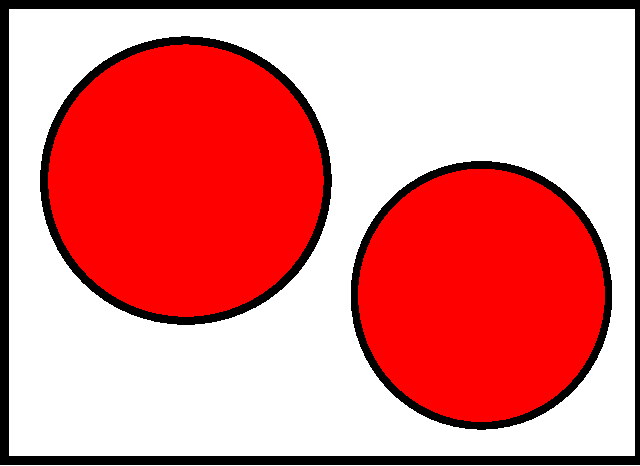
\includegraphics[width=4cm]{disjoint.pdf}
%	\label{fig:Disjunkt}
%\end{figure}

Vi kan nu skapa m�ngder och tala om vilka element de inneh�ller, men hur kan vi
j�mf�ra tv� m�ngder?
Hur vet vi om tv� m�ngder �r lika?
\begin{definition}
	\label{def:Mangdlikhet}\index{m�ngd!likhet}\index{likhet}
	Vi s�ger att tv� m�ngder \(A\) och \(B\) �r \emph{lika} om varje element i
	\(A\) �ven tillh�r \(B\) och varje element i \(B\) �ven tillh�r \(A\).
	Om \(A\) och \(B\) �r lika skriver vi \(A=B\), annars skriver vi \(A\neq
	B\).
\end{definition}
\begin{exercise}
	Unders�k vad detta inneb�r, vilka m�ngder �r egentligen lika?
	�r \(\{1,2,3\}\) lika med \(\{1,1,3,3,2,3,2,1\}\)?
\end{exercise}
\begin{exercise}
	I inledning sades att en m�ngd kan inneh�lla andra m�ngder.
	En m�ngd \(X\) som tillh�r en m�ngd \(M\) �r d� ett element som alla andra i
	m�ngden \(M\).
	Om \(X=\{1,2\}\) och \(M=\{X, 2, 3\}=\{\{1,2\},2,3\}\), vilka av f�ljande
	utsagor �r sanna och vilka �r falska: 
	\(1\in M\), \(2\in M\) och \(3\in M\) samt \(\{1\}\in M\),
	\(\{2\}\in M\) och \(\{1,2\}\in M\).
\end{exercise}
\begin{exercise}
	P� hur m�nga s�tt kan man egentligen matematiskt beskriva den tomma
	m�ngden?
\end{exercise}

Vi forts�tter med ett annat viktigt begrepp.
\begin{definition}
	\label{def:Disjunkt}\index{disjunkt}
	Tv� m�ngder \(A\) och \(B\) s�gs vara \emph{disjunkta} om varje element i
	\(A\) ej �r ett element i \(B\).
\end{definition}
\begin{exercise}
	Om \(A\) och \(B\) �r m�ngder, betyder det samma sak att \(A\neq B\) som
	att \(A\) och \(B\) �r disjunkta?
\end{exercise}
%M�ngderna i \figref{fig:Disjunkt} �r disjunkta.
%M�ngderna i \figref{fig:IckeDisjunkt} �r inte det.
%\begin{figure}[h]
%	\caption{Tv� icke disjunkta m�ngder.}
%	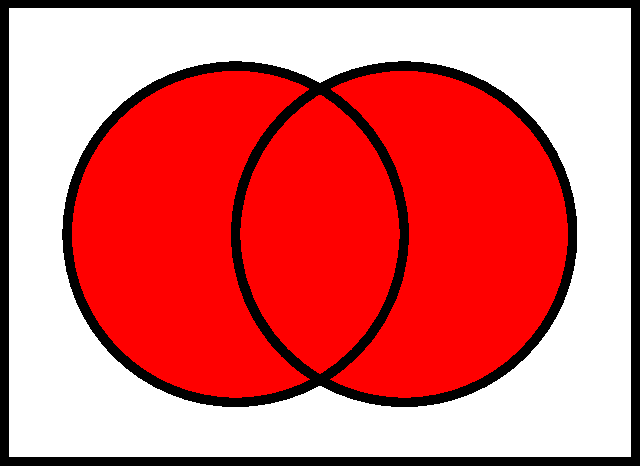
\includegraphics[width=4cm]{union.pdf}
%	\label{fig:IckeDisjunkt}
%\end{figure}


%%%%%%%%%%%%%%%%%%%%%%%%%%%%%%%%%%%%%%%%%%%%
% OPERATIONER P� M�NGDER
%%%%%%%%%%%%%%%%%%%%%%%%%%%%%%%%%%%%%%%%%%%%
\section{Operationer p� m�ngder}
\label{sec:Mangdoperationer}
\noindent
\lettrine{E}{fter att ha} tittat p� vad en m�ngd �r och hur vi kan avg�ra om
tv� m�ngder �r lika ska vi nu titta p� hur vi kan skapa nya m�ngder genom att
kombinera m�ngder som vi redan har.

\begin{definition}
	\label{def:Union}\index{union}
	L�t \(A\) och \(B\) vara m�ngder.
	Vi l�ter m�ngden \(A\cup B\) av alla element i \(A\) och alla element i
	\(B\) kallas f�r \emph{unionen} av \(A\) och \(B\).
	Det vill s�ga, \(A\cup B = \{x : x\in A\tor x\in B\}\).
\end{definition}

%\begin{figure}[h]
%	\caption{Unionen av tv� m�ngder.}
%	\subfloat[M�ngden \(A\).]{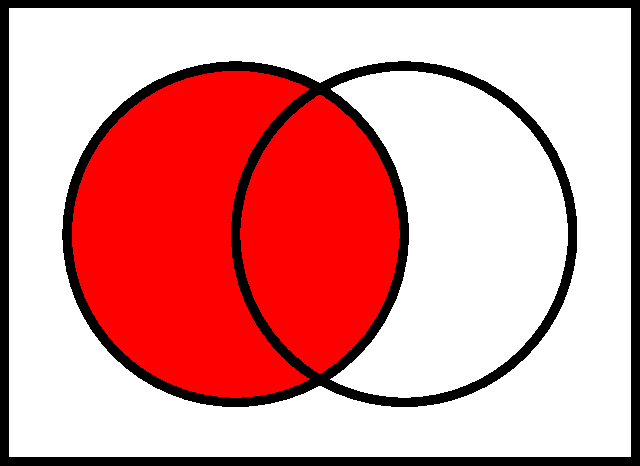
\includegraphics[width=4cm]{A.pdf}}
%	\subfloat[M�ngden \(B\).]{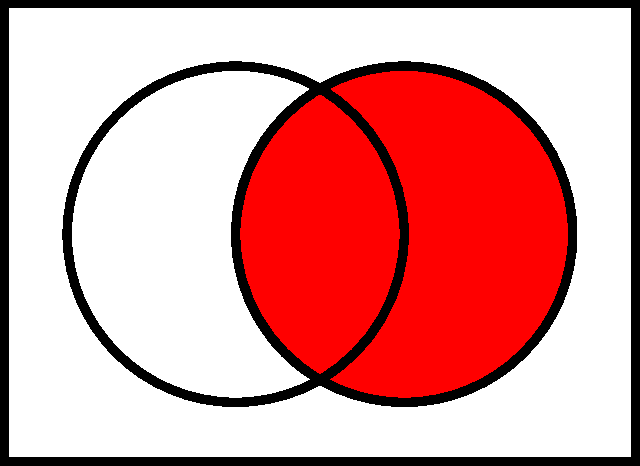
\includegraphics[width=4cm]{B.pdf}}
%	\subfloat[M�ngden \(A\cup B\).]{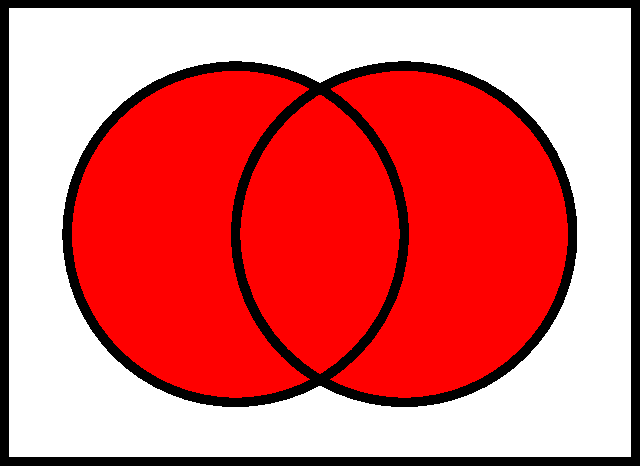
\includegraphics[width=4cm]{union.pdf}}
%	\label{fig:Union}
%\end{figure}

\begin{exercise}
	Utforska unionsbegreppet, finns det n�gra intressanta resultat om detta?
\end{exercise}

\begin{definition}
	\label{def:Snitt}\index{snitt}
	L�t \(A\) och \(B\) vara m�ngder.
	Vi l�ter m�ngden \(A\cap B\) av alla element i \(A\) som ocks� tillh�r
	\(B\) kallas f�r \emph{snittet} mellan \(A\) och \(B\).
	Det vill s�ga, \(A\cap B = \{x : x\in A\tand x\in B\}\).
\end{definition}

%\begin{figure}[h]
%	\caption{Unionen av tv� m�ngder.}
%	\subfloat[M�ngden \(A\).]{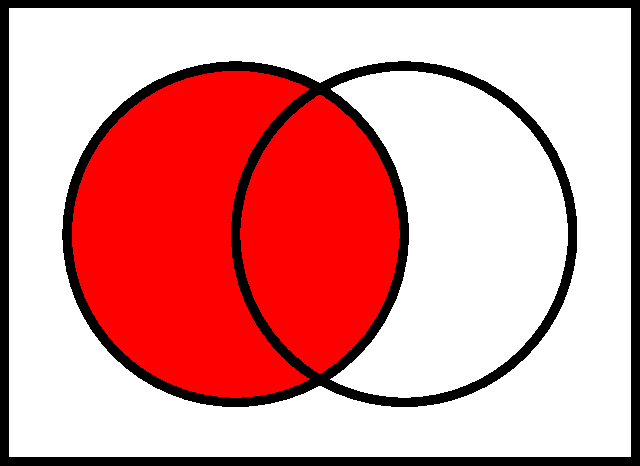
\includegraphics[width=4cm]{A.pdf}}
%	\subfloat[M�ngden \(B\).]{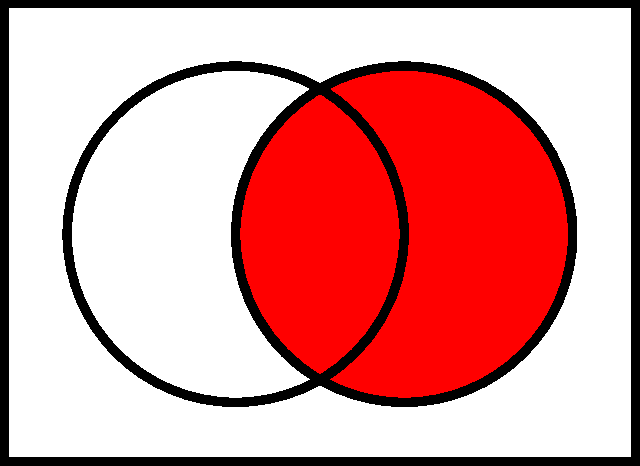
\includegraphics[width=4cm]{B.pdf}}
%	\subfloat[M�ngden \(A\cap B\).]{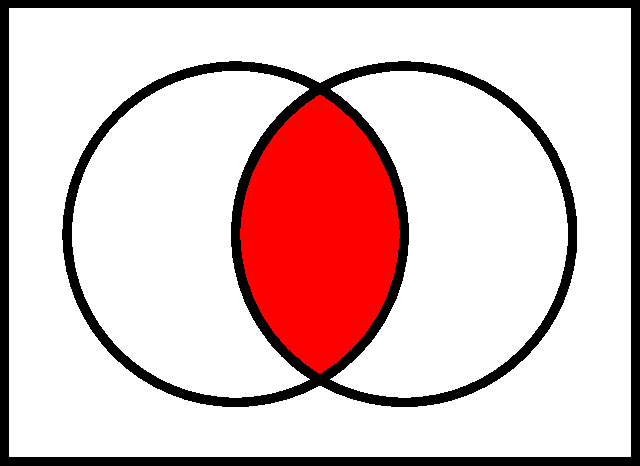
\includegraphics[width=4cm]{intersection.pdf}}
%	\label{fig:Union}
%\end{figure}

\begin{exercise}
	Utforska snittbegreppet, finns det n�gra intressanta resultat om detta?
\end{exercise}

\begin{exercise}
	Hur f�rh�ller sig union- och snittoperationerna? Exempelvis, spelar det
	n�gon roll om vi tar snittet av tv� unioner eller om vi tar unionen av tv�
	snitt?
\end{exercise}

\begin{definition}
	\label{def:Mangddifferens}\index{differens}\index{m�ngd!differens}
	L�t \(A\) och \(B\) vara m�ngder.
	Vi l�ter m�ngden \(A\setminus B\) av alla element i \(A\) som inte tillh�r
	\(B\) kallas f�r \emph{differensen} mellan \(A\) och \(B\).
	Det vill s�ga, \(A\setminus B = \{x : x\in A\tand x\notin B\}\).
\end{definition}

%\begin{figure}[h]
%	\caption{Unionen av tv� m�ngder.}
%	\subfloat[M�ngden \(A\).]{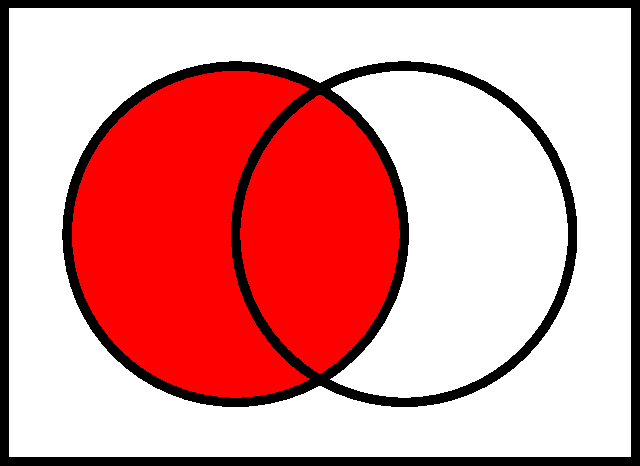
\includegraphics[width=4cm]{A.pdf}}
%	\subfloat[M�ngden \(B\).]{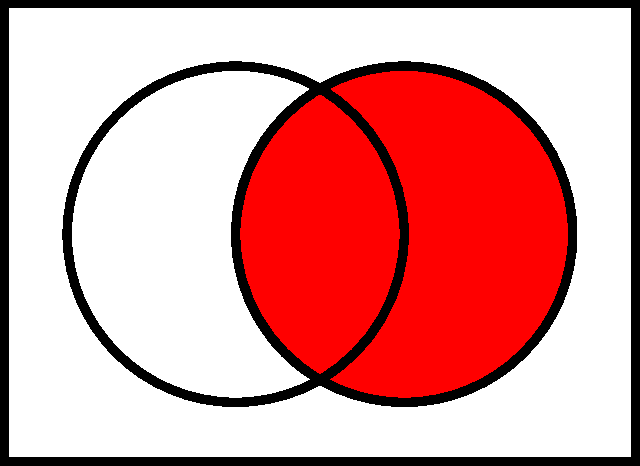
\includegraphics[width=4cm]{B.pdf}}
%	\subfloat[M�ngden \(A\setminus B\).]{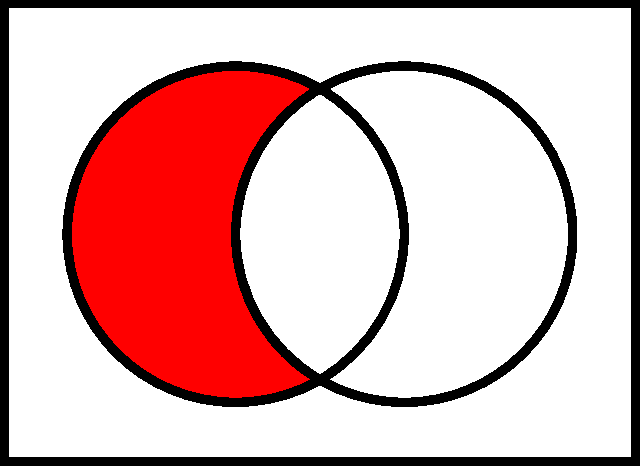
\includegraphics[width=4cm]{A_setminus_B.pdf}}
%	\label{fig:Union}
%\end{figure}

\begin{exercise}
	Finns det n�gra intressanta resultat om differensen? Hur f�rh�ller sig denna
	operation gentemot operationerna union och snitt?
\end{exercise}

\begin{definition}
	\label{def:KartesiskProdukt}\index{kartesisk produkt}
	L�t \(M\) och \(N\) vara m�ngder.
	M�ngden \(\{(m,n) : m\in M\tand n\in N\}\) av alla ordnade par med f�rsta
	element i \(M\) och andra element i \(N\) 
	kallas f�r den \emph{kartesiska produkten} av \(M\) och \(N\) och skrivs
	\(M\times N\).
\end{definition}
Namnet kartesisk produkt kommer fr�n den franske matematikern och filosofen
Ren� Descartes (1596-1650) vars latinska namn var Renatus Cartesius.
Descartes matematiska studier gav upphov till denna typ av begrepp och d�rf�r
�r den kartesiska produkten i efterhand uppkallad efter honom.

\begin{exercise}
	\label{xrc:Kortlek}
	L�t \(V\) vara m�ngden av alla val�rer i en kortlek, det vill s�ga
	\(V=\{2,3,4,5,6,7,8,9,10,\text{knekt},\text{dam},\text{kung},\text{ess}\}\).
	L�t ocks� \(F\) vara m�ngden av f�rger i en kortlek, det vill s�ga
	\(F=\{\spadesuit,\clubsuit,\heartsuit,\diamondsuit\}\).
	Vad blir \(F\times V\) och vad skulle denna m�ngd kunna anv�ndas f�r att
	representera?
\end{exercise}


%%%%%%%%%%%%%%%%%%%%%%%%%%%%%%%%%%%%%%%%%%%%
% DELM�NGDER
%%%%%%%%%%%%%%%%%%%%%%%%%%%%%%%%%%%%%%%%%%%%
\section{Delm�ngder}
\label{sec:Delmangder}
\noindent
\lettrine{H}{�rn�st ska vi} titta p� delar av m�ngder, eller m�ngder vars
element utg�r en del av de element som finns i en annan m�ngd.
Detta �r intressant f�r att det �r inte alltid som vi �r intresserade av hela
m�ngden, det �r inte heller alltid som vi bara �r intresserade av enbart ett
element.
Ibland kan det vara intressantare att titta p� en del av elementen i en m�ngd,
och fr�n dessa skapa en ny m�ngd.
Vi ger d�rf�r f�ljande definition.

\begin{definition}
	\label{def:Delmangd}\index{delm�ngd}
	L�t \(A\) och \(B\) vara m�ngder.
	Vi s�ger att \(A\) �r en \emph{delm�ngd} av \(B\) om varje element i \(A\)
	�ven tillh�r \(B\).
	Vi skriver detta som \(A\subseteq B\) och utl�ser det som att \emph{\(A\)
	�r inkluderad i \(B\)}.
	Vi kan likv�rdigt skriva \(B\supseteq A\) och utl�ser detta som att
	\emph{\(B\) inkluderar \(A\)}.
	Om dessutom \(A\neq B\) �r \(A\) en \emph{�kta} eller \emph{proper
	delm�ngd} av \(B\) och detta skrivs \(A\subset B\) respektive
	\(B\supset A\).
\end{definition}

%\begin{figure}[h]
%	\caption{Tv� m�ngder, d�r den ena �r inkluderad av den andre.}
%	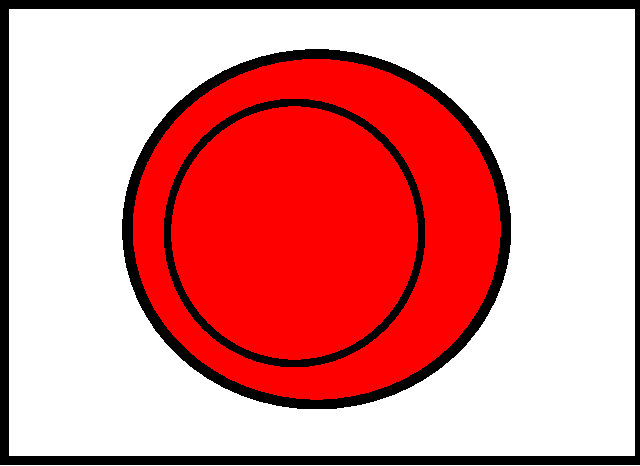
\includegraphics[width=4cm]{subset.pdf}
%	\label{fig:Delmangd}
%\end{figure}

\begin{exercise}
	Vad skulle det inneb�ra om \(A\) �r en delm�ngd av \(B\) och \(B\) �r en
	delm�ngd av \(A\), det vill s�ga \(A\subseteq B\) och \(B\subseteq A\)?
	�r detta ens m�jligt?
	Det �r faktiskt s� att det �r en vanlig bevismetod inom matematiken att
	f�rst visa \(A\subseteq B\) och sedan visa \(B\subseteq A\).
\end{exercise}

Vi forts�tter med en annan definition med koppling till delm�ngdsbegreppet.
\begin{definition}
	\label{def:Komplement}\index{komplement}
	L�t \(A\) vara en delm�ngd till m�ngden \(B\).
	Vi kallar m�ngden \(A^\complement = B\setminus A\) f�r \emph{komplementet}
	till \(A\) i m�ngden \(B\).
\end{definition}

%\begin{figure}[h]
%	\caption{Komplementet till en delm�ngd.}
%	
\includegraphics[width=4cm]{complement.pdf}
%	\label{fig:Komplement}
%\end{figure}

\begin{exercise}
	Vad �r det f�r skillnad mellan begreppen komplement och differens?
\end{exercise}

\begin{example}
	L�t \(M=\{1,2,3\}\) och \(A=\{1,2\}\) vara tv� m�ngder.
	D� har vi att \(A\subseteq M\), det vill s�ga \(A\) �r en delm�ngd till
	\(M\), och faktiskt \(A\subset M\), det vill s�ga \(A\) �r en �kta delm�ngd
	till \(M\).
	Vi har dessutom att komplementet till \(A\) �r \(A^\complement =
	M\setminus A = \{3\}\).
\end{example}

Nu n�r vi har delm�ngder till en m�ngd \(M\), d� kan det vara sk�nt att ha ett
enkelt notationss�tt f�r m�ngden av alla delm�ngder till \(M\).
Denna m�ngd som inneh�ller alla delm�ngder till \(M\) som element kallas
\emph{potensm�ngd} och definieras h�rn�st.
\begin{definition}
	\label{def:Potensmangd}\index{potensm�ngd}
	L�t \(M\) vara en m�ngd.
	Vi kallar m�ngden av alla delm�ngder till \(M\) f�r \emph{potensm�ngden}
	av \(M\).
	Vi betecknar potensm�ngden till \(M\) som \(\powerset(M)\).
\end{definition}
\begin{exercise}
	Unders�k hur potensm�ngden av en m�ngd \(M\) f�rh�ller sig till m�ngden
	\(M\) sj�lv.
\end{exercise}


%%%%%%%%%%%%%%%%%%%%%%%%%%%%%%%%%%%%%%%%%%%%
% RELATIONER
%%%%%%%%%%%%%%%%%%%%%%%%%%%%%%%%%%%%%%%%%%%%
\section[Relationer]{Relationer\maybeskip}
\label{sec:MangderRelationer}
\noindent
\lettrine{V}{i ska nu } titta p� hur vi kan uppr�tta relationer mellan
elementen i en m�ngd.
I tidigare avsnitt har vi redan st�tt p� en relation -- likheten mellan tv�
m�ngder.

\begin{definition}
	\label{def:BinarRelation}\index{relation}\index{bin�r relation}
	En \emph{bin�r relation} \(R\) p� en m�ngd \(M\) �r en delm�ngd till den
	kartesiska produkten \(M\times M\).
	Om \((x,y)\in M\times M\) tillh�r \(R\) skriver vi \(x R y\) som utl�ses
	\emph{\(x\) �r relaterat till \(y\) via \(R\)}.
\end{definition}

\begin{remark}
	M�ngden \(R\) �r f�ljdaktligen en delm�ngd till den kartesiska produkten
	\(M\times M\).
\end{remark}

Enligt denna definition skulle likhetsrelationen mellan m�ngder vara en
relation p� m�ngden av alla m�ngder och tv� m�ngder i denna m�ngd �r relaterade
om de uppfyller kraven i \defref{def:Mangdlikhet}.
Vi ska titta p� ett mindre abstrakt exempel.
\begin{example}
	L�t \(S\) vara m�ngden av alla personer som �r skrivna p� en adress i
	Sverige.
	Tv� personer \(p\in S\) och \(q\in S\) �r relaterade via relationen \(G\)
	om de bor p� samma gata.
	Om \(p\) bor p� ''Gatuv�gen 1, 123\,45 Kommunen'' och \(q\) bor p�
	''Gatuv�gen 3, 123\,45 Kommunen'', d� g�ller att \(p G q\) eftersom att
	b�da bor p� ''Gatuv�gen''.

	Vi kan d� ocks� beskriva \(G\) p� f�ljande vis.
	L�t \(V_i\) vara m�ngden av alla personer som �r skriva p� n�gon v�g \(i\).
	D� �r \(G\) unionen av \(V_i\times V_i\) f�r alla v�gar \(i\) i Sverige.
\end{example}

\begin{exercise}
	Anv�nd m�ngderna som definieras i \xrcref{xrc:Kortlek} och definiera en
	relation f�r n�gon dessa.
	Inspiration: Du kan utg� fr�n ditt favoritkortspel och definiera en eller
	flera l�mpliga relationer mellan kort eller m�ngder av kort.
\end{exercise}


%%%%%%%%%%%%%%%%%%%%%%%%%%%%%%%%%%%%%%%%%%%%
% EKVIVALENSKLASS
%%%%%%%%%%%%%%%%%%%%%%%%%%%%%%%%%%%%%%%%%%%%
\subsection{Ekvivalensrelation och ekvivalensklass}
\noindent
Vi ska nu titta p� en speciell typ av relation -- ekvivalensrelationen.
Ekvivalensrelationen har en s�rskild struktur f�r hur element �r relaterade
till varandra.
Den har sitt namn fr�n att den p�minner om likhetsbegreppet som vi tagit upp
tidigare.

\begin{definition}
	\label{def:Ekvivalensrelation}\index{ekvivalensrelation}
	\index{relation!ekvivalensrelation}
	En bin�r relation \(R\) p� en m�ngd \(M\) som uppfyller att
	\begin{enumerate}
		\item f�r alla \(x\in M\) g�ller att \(x R x\) (reflexivitet),
		\item f�r alla \(x,y\in M\) g�ller att om \(x R y\) d� g�ller �ven
			\(y R x\) (symmetri),
		\item f�r alla \(x,y,z\in M\) g�ller att om \(x R y\) och \(y R z\)
			d� g�ller �ven att \(x R z\) (transitivitet),
	\end{enumerate}
	kallas f�r \emph{ekvivalensrelation}.
\end{definition}
\begin{exercise}
	Unders�k vilka relationer du k�nner till som �r reflexiva, symmetriska och
	transitiva, och f�ljdaktligen �r ekvivalensrelationer.
\end{exercise}

En ekvivalensrelation \emph{partitionerar} en m�ngd \(M\) i disjunkta
delm�ngder kallade partitioner.
Dessa partitioner utg�rs av n�got som brukar
kallas f�r ekvivalensklasser. %, som �r disjunkta delm�ngder av m�ngden \(M\).
\begin{definition}
	\label{def:Ekvivalensklass}\index{ekvivalensklass}
	\index{ekvivalensrelation!ekvivalensklass}
	L�t \(R\) vara en ekvivalensrelation definierad p� m�ngden \(M\).
	Om \(a\) �r ett element i \(M\), d� kallar vi m�ngden
	\(\{x\in M : x R a\}\) f�r \emph{ekvivalensklassen} f�r \(a\) och betecknar
	denna som \([a]_R\), elementet \(a\) s�gs vara en \emph{representant} f�r
	ekvivalensklassen.
\end{definition}
Om det �r klart under vilken relation ekvivalensklassen g�ller r�cker det med
att skriva \([a]\) ist�llet f�r \([a]_R\).

P� samma s�tt som att det g�r att skapa en partition genom att inf�ra en
ekvivalensrelation p� m�ngden g�r det ocks� att skapa en ekvivalensrelation p�
m�ngden genom att partitionera den.

\begin{example}
	L�t \(F\) vara m�ngden av alla f�glar.
	Vi inf�r en relation \(A\) d�r tv� f�glar \(x\) och \(y\) �r relaterade via
	\(A\) om de tillh�r samma f�gelart.
	�r detta en ekvivalensrelation?
	Om \(x\) �r en berguv (\emph{Bubo bubo}), d� m�ste \(x A x\) eftersom att
	\(x\) tillh�r samma f�gelart som sig sj�lv.
	S�ledes �r relationen reflexiv.
	Om \(x\) �r en berguv och om \(x A y\), d� m�ste �ven \(y\) vara en berguv
	och f�ljdaktligen \(y A x\).
	Relationen �r d�rf�r symmetrisk.
	Om \(x\) �r en berguv och \(x A y\), d� m�ste \(y\) vara en berguv.
	Om dessutom \(y A z\) m�ste \(z\) ocks� vara en berguv.
	Eftersom b�de \(x\) och \(z\) �r berguvar g�ller att \(x A z\).
	D� �r relationen transitiv.
	Relationen uppfyller kraven f�r en ekvivalensrelation och m�ste
	d�rf�r vara en ekvivalensrelation.

	Eftersom att relationen \(A\) �r en ekvivalensrelation inneb�r det att den
	partitionerar m�ngden \(F\) av alla f�glar.
	Varje partition, eller ekvivalensklass, �r en m�ngd av alla f�glar inom
	samma art.
	Exempelvis �r m�ngden av alla berguvar en ekvivalensklass.
\end{example}

%\begin{figure}[t]
%	
\includegraphics[width=5cm]{set_partition.pdf}
%	\caption{En m�ngd (hela cirkeln) som �r partitionerad i sex delar. Varje
%	del (f�rg) representerar en ekvivalensklass.}
%\end{figure}

M�ngden av alla ekvivalensklasser hos \(M\) under relationen \(\sim\)
brukar betecknas \(M/\!\sim\) och kallas f�r \emph{kvotm�ngden av \(M\)
och \(\sim\)}\index{kvotm�ngd}.
Om \(m\) �r ett element i \(M\), d� �r \([m]_\sim\) ett element i kvotm�ngden
\(M/\!\sim\).


%%%%%%%%%%%%%%%%%%%%%%%%%%%%%%%%%%%%%%%%%%%%
% AVBILDNINGAR
%%%%%%%%%%%%%%%%%%%%%%%%%%%%%%%%%%%%%%%%%%%%
\section{Avbildningar}
\noindent
\lettrine{V}{i ska nu} inf�ra ett annat v�ldigt centralt begrepp inom
matematiken.
Vi ska titta p� avbildningar, eller funktioner som kanske �r det mer k�nda
namnet.
Funktioner kommer att komma tillbaka senare i kursen.
Vi b�rjar med att definiera vad en funktion �r.

\begin{definition}
	\label{def:Avbildning}\index{avbildning}\index{funktion}
	L�t \(A\) och \(B\) vara m�ngder.
	En \emph{funktion}, eller \emph{avbildning}, \(f\colon A\to B\) tilldelar
	till varje \(a\in A\) ett v�lbest�mt \(b\in B\).
	Vi skriver \(f(a)=b\) eller \(a\mapsto b\) och s�ger att \(a\)
	\emph{avbildas} p� \(b\) eller att \(b\) �r \emph{bilden} av \(a\).
	M�ngden \(A\) s�gs vara funktionens \emph{definitionsm�ngd} och m�ngden
	\(B\) s�gs vara funktionens \emph{v�rdem�ngd}.
\end{definition}
\begin{remark}
	Notera att varje funktion \(f\colon A\to B\) ger en funktionsgraf \(G_f\)
	som �r en delm�ngd till den kartesiska produkten \(A\times B\).
	Det vill s�ga, \(G_f=\{(a,b)\in A\times B : f(a)=b\}\).
	D� �r \((a,b)\in G_f\) om \(f(a)=b\), eller \(a\mapsto b\).
\end{remark}
\begin{example}
	L�t \(A=\{1,2,3\}\) och \(B=\{x,y,z\}\) vara m�ngder.
	Vi l�ter \(f:A\to B\) vara en funktion fr�n \(A\) till \(B\).
	Vi l�ter \(1\mapsto x\), \(2\mapsto z\) och \(3\mapsto y\).
	Vi har d� exempelvis att \(2\) avbildas p� \(f(2)=z\).
\end{example}

\begin{exercise}
	Skulle en funktion kunna ses som en relation?
\end{exercise}

I de flesta fall �r det inte l�mpligt att lista alla avbildningarna f�r
funktionen, det vill s�ga ge dess funktionsgraf, som vi gjorde ovan.
Ist�llet �r det b�ttre att ge en beskrivning av hur elementen ska avbildas.
Vi ska illustrera med tv� exempel.
\begin{example}
	L�t \(M\) vara m�ngden av alla m�nniskor i Sverige och \(P\) vara m�ngden
	av alla geografiska platser p� jorden.
	L�t \(p\colon M\to P\) vara en avbildning fr�n \(M\) till \(P\).
	Vi avbildar d� varje m�nniska i \(M\) p� den geografiska plats i \(P\) d�r
	den f�ddes.
\end{example}
\begin{example}
	L�t \(f\colon M\to M\) vara en avbildning fr�n m�ngden
	\(M=\{0,1,2,3,\ldots\}\) till sig sj�lv, och l�t \(x\) avbildas p�
	\(f(x)=x+1\).
\end{example}

Vi ska nu inf�ra en egenskap f�r avbildningar.
Vi vill kunna beskriva en funktion som avbildar element p� ett s�rskilt vis.
\begin{definition}
	\label{def:Injektiv}\index{injektiv}
	L�t \(f\) vara en funktion fr�n en m�ngd \(A\) till en m�ngd \(B\).
	Vi s�ger att \(f\) �r \emph{injektiv} om f�r varje \(x\in A\) och \(y\in
	A\) g�ller att om \(f(x)=f(y)\) d� �r �ven \(x=y\).
\end{definition}
\begin{example}
	\label{ex:Surjektiv}
	L�t \(A=\{1,2,3\}\) och \(B=\{a,b\}\) vara m�ngder samt l�t \(f\) vara en
	funktion fr�n \(A\) till \(B\).
	Vi l�ter \(f(1)=a\), \(f(2)=b\) och \(f(3)=b\).
	D� �r \(f\) inte injektiv eftersom att \(f(2)=f(3)\) men \(2\neq 3\).
\end{example}
\begin{example}
	\label{ex:Injektiv}
	L�t \(A=\{1,2\}\) och \(B=\{a,b,c\}\) vara m�ngder samt l�t \(f\) vara en
	funktion fr�n \(A\) till \(B\).
	Vi l�ter \(f(1)=a\) och \(f(2)=b\).
	D� �r \(f\) injektiv eftersom att det f�r alla element \(x\in A\) g�ller
	att om \(f(x)=f(y)\) d� �r \(x=y\).
\end{example}

%\begin{figure}[h]
%	\caption{En injektiv funktion fr�n en m�ngd \(X=\{1,2,3\}\) till en m�ngd
%	\(Y=\{A,B,C,D\}\).}
%	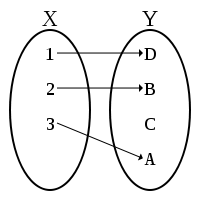
\includegraphics[4cm]{injection.png}
%	\label{fig:Injektion}
%\end{figure}

Vi ska inf�ra en till egenskap likt den ovan.
\begin{definition}
	\label{def:Surjektiv}\index{surjektiv}
	L�t \(f\) vara en funktion fr�n en m�ngd \(A\) till en m�ngd \(B\).
	Vi s�ger att \(f\) �r \emph{surjektiv} om det f�r varje \(b\in B\)
	existerar ett \(a\in A\) s�dant att \(b=f(a)\).
\end{definition}
\begin{example}
	Funktionen \(f\) i \exref{ex:Surjektiv} �r surjektiv eftersom att det f�r
	varje element \(y\in B\) finns ett element i \(x\in A\) s�dant att
	\(f(x)=y\).
\end{example}
\begin{example}
	Funktionen \(f\) i \exref{ex:Injektiv} �r ej surjektiv eftersom att det 
	finns ett element i \(B\), n�mligen \(c\), s�dant att \(f(x)\neq c\) f�r
	alla \(x\in A\).
\end{example}

%\begin{figure}[h]
%	\caption{En surjektiv funktion fr�n en m�ngd \(X=\{1,2,3,4\}\) till en
%	m�ngd \(Y=\{B,C,D\}\).}
%	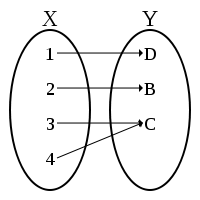
\includegraphics[4cm]{surjection.png}
%	\label{fig:Surjektion}
%\end{figure}

\begin{definition}
	En avbildning som �r b�de injektiv och surjektiv s�gs vara
	\emph{bijektiv}\index{bijektiv}.
\end{definition}



%%%%%%%%%%%%%%%%%%%%%%%%%%%%%%%%%%%
% KARDINALITET
%%%%%%%%%%%%%%%%%%%%%%%%%%%%%%%%%%%
\section{Kardinalitet}
\noindent
\lettrine{V}{i kan avg�ra} om tv� m�ngder �r lika genom att unders�ka om alla
element finns med i b�da m�ngderna, om de g�r det s� �r m�ngderna lika.
Om det d�remot saknas element kan vi i nul�get inte s�ga mycket mer �n att
m�ngderna �r olika.
Det kan dock vara intressant att kunna se hur tv� disjunkta m�ngder f�rh�ller
sig till varandra.
Till exempel genom att best�mma hur stora de �r.

N�r vi avg�r hur stort n�gonting �r, med avseende p� antal, brukar vi r�kna
antalet objekt.
Om vi exempelvis skulle avg�ra hur m�nga personer vi ser just nu b�rjar vi med
att peka p� en person och s�ga \emph{ett}, peka p� en annan person och s�ga
\emph{tv�}, och s� vidare tills att vi har pekat p� samtliga personer vi kan se.
Det vi egentligen g�r n�r vi r�knar p� detta vis �r att uppr�tta en avbildning
fr�n talen \(1,2,3,\ldots\) till objekten vi r�knar.
Vi kan utifr�n denna id� definiera storleken f�r m�ngder, kallad en m�ngds
\emph{kardinalitet}, p� f�ljande vis.
\begin{definition}
	\label{def:Kardinalitet}\index{kardinalitet}
	Om \(A\) och \(B\) �r m�ngder s�ger vi att de har samma \emph{kardinalitet}
	om det finns en bijektiv avbildning mellan \(A\) och \(B\).
	Vi skriver d� att \(\card A = \card B\).
	Om \(A\) har samma kardinalitet som m�ngden \(\{1,2,3,\ldots,n\}\) f�r
	n�got heltal \(n\) skriver vi \(\card A = n\).
	Den tomma m�ngden \(\emptyset\) har kardinalitet \(\card\emptyset = 0\).
\end{definition}

\begin{example}
	M�ngderna \(M=\{a,b,c\}\) och \(N=\{1,2,3\}\) har samma kardinalitet,
	n�mligen \(3\).
	Detta eftersom att avbildningen \(f\colon M\to N\) s�dan att \(f(a)=1\),
	\(f(b)=2\) och \(f(c)=3\) �r bijektiv.
\end{example}

Anledningen till att vi definierar kardinalitet p� detta vis och inte n�jer oss
med att bara r�kna elementen i m�ngden �r f�r att det inte l�ngre g�r att r�kna
elementen n�r m�ngderna blir o�ndligt stora.
Men trots att de �r o�ndligt stora vill vi fortfarande kunna j�mf�ra dem.
Det var just detta som Cantor gjorde, och vi har redan i inledningen n�mnt
n�gra av de resultat som han kom fram till.

%\chapter{Funktioner\maybeskip[Kapitlet �r med enbart f�r att visa
dispositionen.]}
\label{ch:Funktioner}
\noindent
...

\begin{definition}[Funktion]
	...
\end{definition}

\chapter{De naturliga talen}
\noindent
\lettrine{D}{e naturliga talen} �r talen \(0,1,2,3\ldots\) som vi oftast
anv�nder f�r att ordna och r�kna saker med.
M�ngden av naturliga tal betecknas \(N\).

Under 1800-talet blev matematiker uppm�rksamma p� att det beh�vdes en stadigare
grund att bygga matematiken p�.
Under 1800-talets slut och b�rjan av 1900-talet grundades de delar av
matematiken som anv�nts sedan �rtusenden tillbaka.
Richard Dedekind (1831-1916) publicerade 1888 ett antal axiom f�r de naturliga
talen.
�ret efter publicerade Giuseppe Peano (1858-1932) en f�rb�ttring av dessa
axiom och det �r Peanos f�rb�ttrade axiom som godtagits och anv�nds idag,
om �n i lite annorlunda formulering.

Vi ska �ven se i \secref{sec:vonNeumannNaturliga} att Peanos axiom
faktiskt kan h�rledas ur m�ngdteorin och att m�ngdteorin d�rf�r kan anv�ndas
som fundamental teori f�r matematiken.
Dedekind-Peanos axiom kan �nd� anv�ndas som grund f�r de naturliga talen,
ist�llet f�r att vara axiom �r de satser som kan h�rledas i m�ngdteorin.

\section{Dedekind-Peanos axiom f�r de naturliga talen}
\noindent
\lettrine{V}{i ska nu} titta p� Peanos axiom f�r de naturliga talen.
F�r enkelhet av notation l�ter vi \(S\) vara en funktion s�dan att given ett
\(n\) ger den dess efterf�ljare.
Efterf�ljaren betecknas \(S(n)\).
\begin{definition}
	\label{def:DedekindPeano}\label{def:NaturligaAxiom}
	F�r de naturliga talen antas f�ljande axiom:
	\begin{enumerate}
		\item\label{def:NaturligaAxiomNoll}
			\(0\) �r ett naturligt tal. 
		\item\label{def:NaturligaAxiomReflexivitet}
			F�r alla naturliga tal \(n\) g�ller att \(n=n\).
			(Reflexivitet)
		\item\label{def:NaturligaAxiomSymmetri}
			F�r alla naturliga tal \(a\) och \(b\) g�ller att
			om \(a=b\) d� �r \(b=a\).
			(Symmetri)
		\item\label{def:NaturligaAxiomTransitivitet}
			F�r alla naturliga tal \(a,b\) och \(c\) g�ller att
			om \(a=b\) och \(b=c\) d� �r \(a=c\). (Transivitet)
		\item\label{def:NaturligaAxiomSlutenhet}
			F�r alla \(a\) och \(b\) g�ller att om \(a\) �r ett naturligt tal
			och \(a=b\) d� �r \(b\) ocks� ett naturligt tal.
			(Slutenhet under likhet)
		\item\label{def:NaturligaAxiomEfterfoljare}
			F�r alla naturliga tal \(n\) g�ller att efterf�ljaren \(S(n)\) �r
			ett naturligt tal.
		\item\label{def:NaturligaAxiomOandligt}
			F�r alla naturliga tal \(n\) g�ller att \(S(n)\neq 0\).
		\item\label{def:NaturligaAxiomInjektion}
			F�r alla naturliga tal \(a\) och \(b\) g�ller att om \(S(a)=S(b)\)
			d� �r \(a=b\).
		\item\label{def:NaturligaAxiomInduktion}
			Om \(M\) �r en m�ngd s�dan att \(0\) �r ett element i \(M\), och
			f�r alla naturliga tal \(n\) g�ller att om \(n\) �r ett element i
			\(M\) d� �r �ven \(S(n)\) ett element i \(M\).
			d� inneh�ller \(M\) alla naturliga tal.
	\end{enumerate}
	H�refter inf�r vi beteckningarna
	\begin{align*}
		1&=S(0), \\
		2&=S(1)=S(S(0)), \\
		3&=S(2)=S(S(S(0))), \\
		\vdots \\
		n&=S(n-1)=\underbrace{S(S(S(\cdots(S}_n(0))))) = S^n(0).
	\end{align*}
\end{definition}

Det f�rsta axiomet s�ger helt enkelt att det finns ett tal som �r ett naturligt
tal.
Axiomen \ref{def:NaturligaAxiomReflexivitet}, \ref{def:NaturligaAxiomSymmetri},
\ref{def:NaturligaAxiomTransitivitet} och \ref{def:NaturligaAxiomSlutenhet}
behandlar likehet.
Axiomen \ref{def:NaturligaAxiomEfterfoljare},
\ref{def:NaturligaAxiomOandligt} och \ref{def:NaturligaAxiomInjektion}
behandlar talens aritmetiska egenskaper och visar att de �r o�ndligt m�nga.
Det sista axiomet beskriver m�ngden av naturliga tal.



%%%%%%%%%%%%%%%%%%%%%%%%%%%%%%%%%%%%%
% VON NEUMANNS KONSTRUKTION
%%%%%%%%%%%%%%%%%%%%%%%%%%%%%%%%%%%%%
\section{von Neumanns konstruktion av de naturliga talen}
\label{sec:vonNeumannNaturliga}
\noindent
... (i m�n av tid.)



%%%%%%%%%%%%%%%%%%%%%%%%%%%%%%%%%%%%%
% ARITMETIK
%%%%%%%%%%%%%%%%%%%%%%%%%%%%%%%%%%%%%
\section{Aritmetik}
\noindent
...

\begin{definition}
	Ett element \(e\) i en m�ngd med en definierad operation \(\diamond\)
	kallas \emph{identitetselement} om och endast om det f�r alla element
	\(x\) i m�ngden uppfyller att \(x\diamond e=x\).
\end{definition}


%%%%%%%%%%%%%%%%%%%%%%%%%%%%%%%%%%%%%
% ADDITION
%%%%%%%%%%%%%%%%%%%%%%%%%%%%%%%%%%%%%
\subsection{Addition}
\noindent
...

\begin{definition}[Addition]
	\label{def:NaturligaAddition}
	P� de naturliga talen definieras en bin�r operation kallad \emph{addition}
	(\(+\)) som
	\begin{align}
		\label{eq:AdditionNoll}
		a+0 &= a, \\
		\label{eq:AdditionRekursion}
		a+S(b) &= S(a+b).
	\end{align}
\end{definition}
\begin{theorem}\label{thm:NaturligaAdderaEtt}
	Om \(a\) �r ett naturligt tal �r \(a+1\) dess efterf�ljare.
\end{theorem}
\begin{proof}
	Om vi tittar p� additionen \(a+1\) har vi \(a+1=a+S(0)\).
	Fr�n \eqref{eq:AdditionRekursion} f�r vi att \(a+S(0)=S(a+0)\).
	Vi har slutligen fr�n \eqref{eq:AdditionNoll} att \(a+0=a\).
	Vi f�r d� att
	\begin{equation}\label{eq:NaturligaAdderaEtt}
		a+1 = a+S(0) = S(a+0) = S(a).
	\end{equation}
	Allts� �r \(a+1\) efterf�ljaren \(S(a)\) till \(a\).
\end{proof}
\begin{example}
	Om vi vidare tittar p� additionen \(a+2\) har vi att
	\begin{equation*}
		a+2 = a+S(1) = S(a+1).
	\end{equation*}
	Vi har fr�n \thmref{thm:NaturligaAdderaEtt} att \(a+1=S(a)\) och allts�
	f�r vi att
	\begin{equation*}
		a+2=S(S(a))=(a+1)+1.
	\end{equation*}
\end{example}
Vi kan nu formulera en vidareutveckling av detta.
\begin{theorem}
	\label{thm:NaturligaAdderaN}
	Om \(a\) och \(n\) �r naturliga tal g�ller att
	\begin{equation}
		a+n=\underbrace{S(S(S(\cdots(S}_{n}(a)))))=S^n(a).
	\end{equation}
\end{theorem}
\begin{proof}
	Vi har enligt \defref{def:NaturligaAxiom} \(n=S^n(0)\).
	D� har vi att \(a+n=a+S^n(0)\).
	Enligt \eqref{eq:AdditionRekursion} �r \(a+S^n(0) = S(a+S^{n-1}(0))\).
	Men enligt \eqref{eq:AdditionRekursion} �r \(a+S^{n-1}(0)=S(a+S^{n-2}(0))\).
	Vi har allts� att \[a+n=S(S(a+S^{n-2}(0)))=S^2(a+S^{n-2}(0)).\]
	S�ledes har vi \(S^k(a+S^{n-k}(0))\) f�r \(k\leq n\).
	N�r \(k=n\) f�r vi \(S^n(a+S^{n-n}(0)) = S^n(a+0) = S^n(a)\).
\end{proof}

\begin{theorem}[Associativitet]
	Om \(a,b\) och \(c\) �r naturliga tal, d� g�ller att \(a+(b+c)=(a+b)+c\).
\end{theorem}
\begin{proof}
	Vi b�rjar med att titta p� \(a+(b+c)\).
	Enligt \thmref{thm:NaturligaAdderaN} har vi att \(b+c=S^c(b)\).
	Enligt \defref{def:NaturligaAxiom} �r \(b=S^b(0)\) och vi f�r allts� att
	\(b+c=S^c(S^b(0)).\)
	Vi har d� kvar \(a+(b+c)=a+S^c(S^b(0))\).
	Enligt \thmref{thm:NaturligaAdderaN} igen har vi
	\begin{equation}\label{eq:NaturligaAssociativ1}
		a+S^c(S^b(0))=S^c(S^b(a))=S^c(S^b(S^a(0))).
	\end{equation}

	Vi forts�tter med att kolla p� \((a+b)+c\).
	D� har vi \(a+b=S^b(a)\) och s�ledes
	\begin{equation}\label{eq:NaturligaAssociativ2}
		S^b(a)+c=S^c(S^b(a))=S^c(S^b(S^a(0))).
	\end{equation}

	Vi ser att \eqref{eq:NaturligaAssociativ1} och
	\eqref{eq:NaturligaAssociativ2} �r lika och s�ledes har vi �ven att
	\[a+(b+c)=(a+b)+c.\]
\end{proof}

\begin{theorem}[Kommutativitet]
	Om \(a\) och \(b\) �r naturliga tal, d� g�ller att \(a+b=b+a\).
\end{theorem}
\begin{proof}
	Vi har fr�n \thmref{thm:NaturligaAdderaN} att \(a+b=S^b(a)=S^b(S^a(0))\).
	Men
	\begin{equation}
		\label{eq:NaturligaKommutativ1}
		S^b(S^a(0)) =
		\underbrace{S(S(S(\cdots(S}_b(\underbrace{S(S(S(\cdots(S}_a(0)))))))))).
	\end{equation}

	P� samma s�tt har vi att \(b+a=S^a(b)=S^a(S^b(0))\) och
	\begin{equation}
		\label{eq:NaturligaKommutativ2}
		S^a(S^b(0)) =
		\underbrace{S(S(S(\cdots(S}_a(\underbrace{S(S(S(\cdots(S}_b(0)))))))))).
	\end{equation}

	Eftersom att \eqref{eq:NaturligaKommutativ1} och
	\eqref{eq:NaturligaKommutativ2} �r lika m�ste vi ha \(a+b=b+a\).
\end{proof}



%%%%%%%%%%%%%%%%%%%%%%%%%%%%%%%%%%%%%
% MULTIPLIKATION
%%%%%%%%%%%%%%%%%%%%%%%%%%%%%%%%%%%%%
\subsection{Multiplikation}
\noindent
...

\begin{definition}[Multiplikation]
	\label{def:NaturligaMultiplikation}
	P� de naturliga talen definieras en bin�r operation \emph{multiplikation}
	(\(\cdot\)) som
	\begin{align}
		a\cdot 0 &= 0 \\
		a\cdot S(b) &= a+(a\cdot b)
	\end{align}
\end{definition}

\begin{theorem}[Associativitet]
	Om \(a\) och \(b\) �r naturliga tal, d� g�ller att \(a\cdot(b\cdot
	c)=(a\cdot b)\cdot c\).
\end{theorem}
\begin{proof}
	...
\end{proof}

\begin{theorem}[Kommutativitet]
	Om \(a\) och \(b\) �r naturliga tal, d� g�ller att \(a\cdot b=b\cdot a\).
\end{theorem}
\begin{proof}
	...
\end{proof}

\begin{theorem}[Distributivitet]
	Om \(a,b\) och \(c\) �r naturliga tal g�ller att
	\(a\cdot(b+c) = a\cdot b + a\cdot c.\)
\end{theorem}
\begin{proof}
	...
\end{proof}


%%%%%%%%%%%%%%%%%%%%%%%%%%%%%%%%%%%%%
% LIKHET OCH OLIKHET
%%%%%%%%%%%%%%%%%%%%%%%%%%%%%%%%%%%%%
\section{Likhet och olikhet}
\noindent
...

\begin{definition}[Ordning]
	...
\end{definition}


%%%%%%%%%%%%%%%%%%%%%%%%%%%%%%%%%%%%%
% N�GRA SATSER F�R DE NATURLIGA TALEN
%%%%%%%%%%%%%%%%%%%%%%%%%%%%%%%%%%%%%
\section{N�gra satser f�r de naturliga talen}
\noindent
...

\begin{theorem}[V�lordningsegenskapen hos de naturliga talen]
	\label{def:Valordningsprincipen}
	Om \(M\subseteq\N\) �r en delm�ngd till de naturliga talen och om
	\(M\neq\emptyset\), d� existerar ett \(m\in M\) s�dant att \(m\leq k\) f�r
	alla \(k\in M\).
\end{theorem}
\begin{proof}
	...
\end{proof}


%%%%%%%%%%%%%%%%%%%%%%%%%%%%%%%%%%%%%
% POTENSER
%%%%%%%%%%%%%%%%%%%%%%%%%%%%%%%%%%%%%
\section{Potenser}
\noindent
...


\chapter{De hela talen}
\label{ch:Heltalen}
\noindent
%\lettrine{M}{�ngden av} hela tal $\Z=\{0, -1, 1, -2, 2, \ldots\}$.
\lettrine{V}{i �r nu} v�lbekanta med de naturliga talen,
\(\N=\{0,1,2,\ldots\}\).
Vi har operationerna addition och multiplikation och vet hur dessa fungerar.
I detta kapitel kommer vi att ut�ka de naturliga talen med avseende p�
addition.

Om vi adderar tv� tal \(a\) och \(b\) f�r vi ett trejde tal \(c\), vi skriver
detta som \(a+b=c\).
Det finns dock inget s�tt att ta oss tillbaka till \(a\), det vill s�ga det
finns inget naturligt tal \(d\) s�dant att \(c+d=a+b+d=a\).
Ett annat s�tt att s�ga det p� �r att det finns inga naturliga tal \(n\) och
\(m\) s�dana att deras summa \(n+m=0\) �r lika med identitetselementet noll.
Detta �r dock en v�ldigt intressant och �nskv�rd egenskap.
Vi ska f�rtydliga vad vi menar och ge denna egenskap ett namn.
\begin{definition}
	\label{def:invers}
	\index{invers}
	Givet en m�ngd med en definierad bin�r operation \(\diamond\) och ett
	identitetselement \(e\).
	Ett element \(b\) kallas f�r \emph{inversen till \(a\)} om
	\(a\diamond b = b\diamond a = e\).
\end{definition}
\begin{exercise}
	Utforska inversbegreppet.
	Fr�gor att inspirera:
	I \defref{def:invers}, �r \(a\) inversen till n�got element?
	Hur m�nga inverser kan ett element ha?
	Har alla element en invers?
\end{exercise}
%\begin{remark}
%	Av inversens natur f�ljer att om \(b\) �r inversen till \(a\), d� �r �ven
%	\(a\) inversen till \(b\).
%\end{remark}

Vi ska i detta kapitel tillf�ra denna egenskap till additionen f�r de naturliga
talen.
Resultatet �r vad som kallas de hela talen, och m�ngden av de hela talen
betecknas\footnote{Anledningen till att de betecknas med \(\Z\) �r tyskans
\emph{Zahlen} som betyder tal (engelskans \emph{numbers}).} \(\Z\).


%%%%%%%%%%%%%%%%%%%%%%%%%%%%%%%%%%%
% UT�KNINGEN
%%%%%%%%%%%%%%%%%%%%%%%%%%%%%%%%%%%
\section{Ut�kningen av de naturliga talen\maybeskip}
\label{sec:HeltalensKonstruktion}
\noindent
\lettrine{L}{�t oss nu} skapa de hela talen.
Det enda vi har att tillg� �r de naturliga talen, dessa vet vi att de
existerar och hur de fungerar.
Vi b�rjar med att l�ta m�ngden \(M = \N\times\N =
\{(a,b) : a\text{ och }b\text{ �r naturliga tal}\}\) vara m�ngden av alla
ordnade par av naturliga tal.
\begin{example}
	Vi har exempelvis att \((1,2)\in M\) och \((2,1)\in M\) samt att
	\((1,2)\neq (2,1)\).
\end{example}

L�t oss nu inf�ra en ekvivalensrelation \(\sim\) p� denna m�ngd.
Om \((a,b)\) och \((c,d)\) �r ordnade par av naturliga tal, det vill s�ga
element i m�ngden \(M\), d� vi vill att \((a,b)\sim (c,d)\) ska vara sant
precis n�r \(a+d=b+c\).
\begin{exercise}
	Kan vi vara s�kra p� att ekvivalensrelationen \(\sim\) faktiskt �r en
	ekvivalensrelation?
\end{exercise}

Vi betecknar ekvivalensklasserna p� f�ljande s�tt:
Om \((a,b)\) �r ett element i \(M\), d� �r
\([(a,b)]=\{(x,y)\in M : (a,b)\sim (x,y)\}\).
Det vill s�ga, \([(a,b)]\) inneh�ller alla talpar i \(M\) som uppfyller
ekvivalensrelationen med talparet \((a,b)\).
\begin{example}
	Vi har att \((0,0)\sim (1,1)\) eftersom att \(0+1 = 0+1\).
	Allts� har vi \([(0,0)]=[(1,1)]\) och \((1,1)\in [(0,0)]\).
\end{example}
\begin{example}
	Vi har d�remot \((0,0)\nsim (1,0)\) eftersom att \(0+0\neq 0+1\).
	Allts� har vi \((1,0)\notin [(0,0)]\).
\end{example}
\begin{remark}
	Kom ih�g att det spelar ingen roll vilket talpar fr�n en ekvivalensklass
	som vi v�ljer som representant.
\end{remark}

L�t oss nu definiera en bin�r operation \(+\) som vi kallar f�r addition och en
bin�r operation \(\cdot\) som vi kallar f�r multiplikation p� m�ngden av
ekvivalensklasser hos \(M\).
\begin{remark}
	M�ngden av ekvivalensklasser under ekvivalensrelationen \(\sim\) p� m�ngden
	\(M\) �r inte densamma som m�ngden \(M\) och brukar normalt betecknas med
	\(M/\sim\).
	M�ngden \(M=\{(a,b) : a \text{ och } b \text{ �r naturliga tal}\}\), det
	vill s�ga \(M\) inneh�ller ordnade par av naturliga tal, medan m�ngden
	av alla ekvivalensklasser �r \(\{[(a,b)] : (a,b)\in M\}\) och allts�
	inneh�ller m�ngder.
\end{remark}
Vi l�ter \([(a,b)]+[(c,d)] = [(a+c, b+d)]\) och \([(a,b)]\cdot [(c,d)] =
[(ac+bd, ad+bc)]\).
\begin{example}
	\label{ex:HeltalAddition}
	Om vi adderar \([(1,2)]\) och \([(2,4)]\) f�r vi
	\begin{equation*}
		[(1,2)]+[(2,4)] = [(1+2,2+4)] = [(3, 6)] = [(0,3)].
	\end{equation*}
\end{example}
\begin{example}
	\label{ex:HeltalMultiplikation}
	Om vi multiplicerar \([(1,2)]\) och \([(2,4)]\) f�r vi
	\begin{equation*}
		[(1,2)]\cdot [(2,4)] = [(1\cdot 2 + 2\cdot 4, 1\cdot 4 + 2\cdot 2)] =
		[(10, 8)] = [(2,0)].
	\end{equation*}
\end{example}

Vi har nu tal med egenskapen att om vi adderar dem f�r vi identitetselementet.
Identitetselementet f�r addition m�ste vara ekvivalensklassen \([(0,0)]\).
\begin{proof}
	Eftersom att \([(a,b)]+[(0,0)] = [(a+0,b+0)] = [(a,b)]\) och
	\([(0,0)]+[(a,b)] = [(0+a,0+b)] = [(a,b)]\) m�ste \([(0,0)]\)
	vara identitetselementet f�r addition.
\end{proof}

Inversen till \([(a,b)]\) �r \([(b,a)]\).
\begin{proof}
	Inversen till \([(a,b)]\) �r \([(b,a)]\) eftersom att
	\([(a,b)]+[(b,a)]=[(a+b,b+a)]=[(a+b,a+b)]\).
	Eftersom att \(0+(a+b)=0+(a+b)\) har vi enligt ekvivalensrelationen att
	\((0,0)\sim (a+b,a+b)\) och allts� m�ste de tillh�ra samma ekvivalensklass.
	Detta inneb�r att \([(a,b)]\) och \([(b,a)]\) m�ste vara varandras inverser.
\end{proof}
Allts� har varje tal �tminstone en invers, vilket var vad vi �nskade.
L�t oss beteckna inversen f�r heltalet \(a\) med \(-a\).

\begin{exercise}
	Kan ett tal ha fler �n en invers?
\end{exercise}

L�t oss nu inf�ra f�ljande enklare beteckningar.
\begin{definition}
	L�t \(0\) beteckna ekvivalensklassen \([(0,0)]\).
	L�t \(1\) beteckna ekvivalensklassen \([(1,0)]\), \(2\) beteckna
	\([(2,0)]\), och s� vidare.
\end{definition}
De nya beteckningarna och ekvivalensklasserna visas i
\figref{fig:HeltalensEkvivalensklasser}.

\begin{exercise}
	I \exref{ex:HeltalAddition}, vilka tal adderades och vilket blev resultatet?
\end{exercise}
\begin{exercise}
	I \exref{ex:HeltalMultiplikation}, vilka tal multiplicerades och vilket
	blev resultatet?
\end{exercise}

\begin{figure}[t]
	\centering
	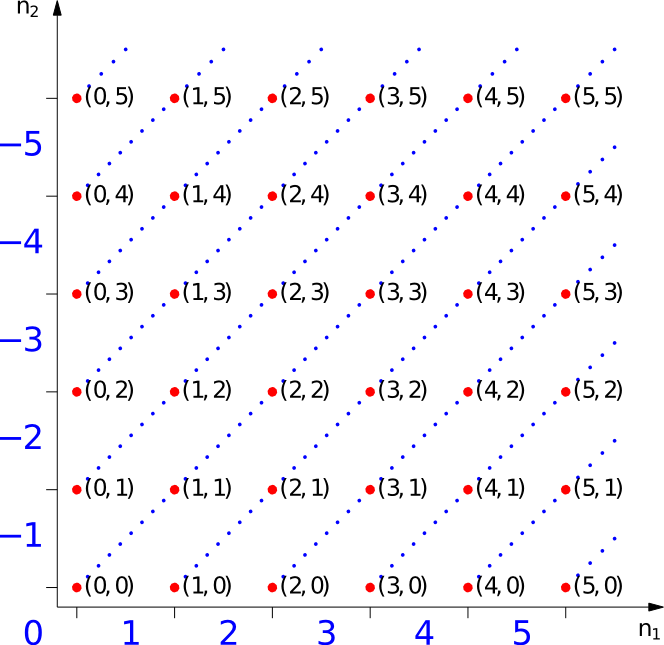
\includegraphics[width=8cm]{Integers_Representation.png}
	\caption{Ekvivalensklasser f�r par av naturliga tal \((n_1,n_2)\) under
		relationen \(\sim\).}
	\label{fig:HeltalensEkvivalensklasser}
\end{figure}

Vi sammanfattar detta avsnitt med f�ljande definitioner.
Vi b�rjar med att definiera vad de hela talen �r.
\begin{definition}[Heltalen]
	\index{heltal}
	L�t \(M=\N\times\N\) vara m�ngden av alla naturliga talpar och \(\sim\)
	vara en ekvivalensrelation p� m�ngden \(M\) s�dan att \((a,b)\sim (c,d)\)
	�r uppfylld f�r element \((a,b)\) och \((c,d)\) i \(M\) om \(a+d=b+c\).

	L�t \(\Z=\{[(a,b)] : (a,b)\in M\}\) vara m�ngden av alla ekvivalensklasser
	f�r \(M\) under ekvivalensrelationen \(\sim\).
	Varje element \(n\) i \(\Z\) kallar vi ett \emph{heltal}.

	L�t ocks� \(0\) beteckna \([(0,0)]\in\Z\), \(1\) beteckna \([(1,0)]\in\Z\)
	och s� vidare.
\end{definition}

N�r vi nu vet vad ett heltal �r kan det vara passande att inf�ra aritmetiska
operationer f�r dem.
Vi b�rjar med additionen, vi tar multiplikationen senare.
\begin{definition}[Addition]
	\index{addition}\index{heltal!addition}
	L�t \(x=[(a,b)]\) och \(y=[(c,d)]\) vara heltal och \(+\) en bin�r
	operation p� \(\Z\), kallad \emph{addition}, s�dan att
	\(x+y=[(a,b)]+[(c,d)]\) �r lika med \([(a+c,b+d)]\).
\end{definition}

Nu n�r vi kan addera heltal �r det l�mpligt att vi tittar p� hur vi kan j�mf�ra
dem annat �n med likhet.
Olikheter inf�rdes med hj�lp av additionen f�r de naturliga talen, det �r inte
f�rv�nande att vi g�r detsamma f�r heltalen.
\begin{definition}[Olikhet]
	\index{olikhet}
	L�t \(x=[(a,b)]\) och \(y=[(c,d)]\) vara heltal.
	Vi s�ger att \(x\) \emph{�r mindre �n} \(y\), betecknat \(x<y\), om
	\(a+d<b+c\).
	Vi kan ocks� s�ga att \(y\) \emph{�r st�rre �n} \(x\) och skriver d�
	\(y>x\).
	Vi s�ger att \(x\) \emph{�r mindre �n eller lika med} \(y\) om \(a+d\leq
	b+c\), detta betecknas \(x\leq y\).
	Vi kan ocks� s�ga att \(y\) \emph{�r st�rre �n eller lika med} \(x\) och
	betecknas \(y\geq x\).
\end{definition}

Den definition som �r den naturliga efterf�ljaren till olikheter �r denna.
\begin{definition}
	\index{negativt tal}\index{positivt tal}
	L�t oss kalla ett tal mindre �n noll f�r ett \emph{negativt} tal, och l�t
	oss kalla ett tal st�rre �n noll f�r ett \emph{positivt} tal.
\end{definition}
Vi har nu inf�rt olika namn f�r talen p� b�da sidorna om talet noll.

Nu till inverserna.
\begin{definition}
	\index{negation}\index{additiv invers}
	Om \(x=[(a,b)]\) �r ett heltal, d� �r \(-x=-[(a,b)]=[(b,a)]\) dess
	\emph{additiva invers}.
	Denna kallas �ven f�r \emph{negationen} av \(x\).
\end{definition}
\begin{remark}
	L�t \(a\) och \(b\) vara heltal och \(-b\) �r den additiva inversen till
	\(b\).
	Normalt skriver vi \(a+(-b)\) som \(a-b\) f�r att spara in p� n�gra tecken.
	Vi ben�mner \(a-b\) som \emph{subtraktionen}\index{subtraktion} av \(b\)
	fr�n \(a\).
	Ur en matematisk synvinkel adderar vi den additiva inversen f�r \(b\) till
	\(a\).
\end{remark}

Den andra aritmetiska operationen, multiplikation, ger vi i den sista
definitionen.
\begin{definition}[Multiplikation]
	\index{multiplikation}\index{heltal!multiplikation}
	L�t \(x=[(a,b)]\) och \(y=[(c,d)]\) vara heltal och \(\cdot\) en bin�r
	operation p� \(\Z\), kallad \emph{multiplikation}, s�dan att
	\(xy=[(a,b)]\cdot [(c,d)]\) �r lika med \([(ac+bd,ab+bc)]\).
\end{definition}

\begin{exercise}
	�r additionen kommutativ f�r de hela talen?
\end{exercise}
\begin{exercise}
	�r additionen associativ f�r de hela talen?
\end{exercise}
\begin{exercise}
	�r multiplikationen kommutativ f�r de hela talen?
\end{exercise}
\begin{exercise}
	�r multiplikationen associativ f�r de hela talen?
\end{exercise}
\begin{exercise}
	�r multiplikationen distributiv �ver additionen f�r de hela talen?
\end{exercise}
\begin{exercise}
	De naturliga talens ordning �r \(0<1<2<3<\ldots\), och s� vidare.
	Hur ordnas de hela talen?
\end{exercise}


%%%%%%%%%%%%%%%%%%%%%%%%%%%%%%%%%%%
% ALGEBRAISKA EGENSKAPER
%%%%%%%%%%%%%%%%%%%%%%%%%%%%%%%%%%%
\section{Algebraiska egenskaper f�r de hela talen}
\label{sec:HeltalensAlgebraiskaEgenskaper}
\noindent
\lettrine{D}{et �r nu dags} att sammanfatta de algebraiska egenskaperna f�r de
hela talen.
De hela talen bygger p� de naturliga talen och ska vara en ut�kning av dessa.
Vi hade f�r avsikt att de hela talen skulle ha samma algebraiska egenskaper som
vi visat att de naturliga talen har.
Vi forts�tter d�rf�r h�rn�st med en sammanfattning av de algebraiska egenskaper
som de hela talen m�ste ha.
Dessa �r desamma som f�r de naturliga talen f�rutom till�gget om att varje tal
\(a\) har en additiv invers \(-a\).

\theoremstyle{plain}
\newtheorem*{AlgebraicPropertiesIntegers}{Algebraiska egenskaper f�r de hela
	talen}
\begin{AlgebraicPropertiesIntegers}
	\nocite{Bartle2000itr,Grillet2007aa}
	\label{def:HeltalenEgenskaper}
	P� m�ngden \(\Z\) av hela tal definieras tv� bin�ra operationer,
	addition (\(+\)) och multiplikation (\(\cdot\)).
	F�r addition g�ller f�ljande:
	\begin{description}
		\item[Kommutativitet] \(a+b=b+a\) f�r alla \(a,b\in\Z\).
		\item[Associtivitet] \((a+b)+c=a+(b+c)\) f�r alla \(a,b,c\in\Z\).
		\item[Additivt identitetselement] Det finns ett element \(0\in\Z\)
			s�dant att f�r alla \(a\in\Z\) g�ller att \(0+a = a+0 = a\).
		\item[Additiv invers] F�r alla \(a\in\Z\) finns ett element \(-a\in\Z\)
			s�dant att \(a + (-a) = (-a) + a = 0\).
	\end{description}
	F�r multiplikation g�ller f�ljande:
	\begin{description}
		\item[Kommutativitet] \(a \cdot b=b \cdot a\) f�r alla \(a,b\in\Z\).
		\item[Associtivitet] \((a \cdot b) \cdot c=a \cdot (b \cdot c)\) f�r
			alla \(a,b,c\in\Z\).
		\item[Multiplikativt identitetselement] Det finns ett element
			\(1\in\Z\) s�dant att f�r alla \(a\in\Z\) g�ller att
			\(1 \cdot a = a \cdot 1 = a\).
	\end{description}
	Ut�ver detta g�ller �ven
	\begin{description}
		\item[Multiplikativ distributivitet �ver addition]
			\(a \cdot (b+c) = (a \cdot b) + (a \cdot c)\) och
			\((b+c) \cdot a = (b \cdot a) + (c \cdot a)\) f�r alla reella tal
			\(a,b,c\in\Z\).
	\end{description}
\end{AlgebraicPropertiesIntegers}



%%%%%%%%%%%%%%%%%%%%%%%%%%%%%%%%%%%%%%%%%%%%
% ALGEBRAISKA EGENSKAPER F�R DE NEGATIVA TALEN
%%%%%%%%%%%%%%%%%%%%%%%%%%%%%%%%%%%%%%%%%%%%
\section{Algebraiska egenskaper f�r de negativa talen}
\noindent
\lettrine{V}{i �r redan} bekanta med de naturliga talen, och allts� med den
delen av de hela talen som motsvarar de naturliga talen.
D�rf�r ska vi i detta avsnitt fokusera p� de nya talen, de heltal \(a<0\) som
�r mindre �n noll -- eller de negativa talen.

L�t oss b�rja med ett av de fundamentala resultaten,
% (-1)a = -a
n�mligen att ett heltal \(a\) multiplicerat med \(-1\) ger dess invers \(-a\).
Vi formulerar detta som en sats.
\begin{theorem}
	\label{thm:FaktoriseraNegativaTal}
	L�t \(a\) vara ett heltal.
	D� �r \(a\) multiplicerat med \(-1\) inversen \(-a\) till \(a\).
	Allts�, \((-1)\cdot a = -a\).
\end{theorem}
\begin{proof}
	Vi har att \(1+(-1) = 0\).
	Om vi multiplicerar noll med ett tal f�r vi fortfarande noll.
	Allts� f�r vi att \(a(1+(-1))=0\) eftersom att vi d� multiplicerar \(a\)
	med noll.
	Eftersom att multiplikation �r distributiv �ver addition f�r vi d� att
	\begin{equation*}
		a(1+(-1)) = 1\cdot a + (-1)a = a + (-1)a = 0.
	\end{equation*}
	D� m�ste \((-1)a\) vara inversen \(-a\) till \(a\).
\end{proof}
\begin{remark}
	Notera att detta och f�ljande resultat �ven kan h�rledas direkt fr�n
	talparskonstruktionen i \secref{sec:HeltalensKonstruktion} trots att vi
	i detta bevis anv�nder oss av de algebraiska egenskaperna givna i
	\secref{sec:HeltalensAlgebraiskaEgenskaper}.
\end{remark}

% (-1)(-1) = (-1)^2 = 1
Vi forts�tter med kanske det mest h�pnanv�ckande resultatet, som �r en
f�ljdsats till f�reg�ende.
\begin{corollary}
	Den additiva inversen \(-1\) till heltalet ett multiplicerad med sig
	sj�lv �r ett.
	Det vill s�ga \((-1)(-1) = 1\).
\end{corollary}
\begin{proof}
	Eftersom att \(-1\) �r ett heltal f�ljer det fr�n
	\thmref{thm:FaktoriseraNegativaTal} att om vi multiplicerar det med \(-1\)
	f�r vi dess invers.
	Inversen f�r \(-1\) �r \(1\) och allts� har vi att \((-1)(-1)=1\).
\end{proof}

L�t oss avsluta med ett exempel om addition av tv� negativa tal.
\begin{example}
	% (-1)+(-1) = -2
	Om vi adderar \(-1\) och \(-1\), vad f�r vi d�?
	Eftersom att vi adderar tv� lika termer kan vi skriva additionen som
	multiplikationen \(2\cdot (-1) = (-1)+(-1)\).
	Vi vet fr�n \thmref{thm:FaktoriseraNegativaTal} att ett heltal
	multiplicerat med \(-1\) �r dess invers, allts� f�r vi \((-1)+(-1)=2\cdot
	(-1) = -2\).
\end{example}
\begin{exercise}
	% (-1)(a+b) = (-a)+(-b)
	Om \(a\) och \(b\) �r heltal,
	g�ller generellt att \((-a)+(-b)=-(a+b)\)?
\end{exercise}

\begin{exercise}
	% (-1)(a-b) = (-1)(a+(-b)) = (-a)+b
	Utred vad \(-(a-b)\) egentligen betyder?
\end{exercise}


%%%%%%%%%%%%%%%%%%%%%%%%%%%%%%%%%%%%%%%%%%%%
% POTENSER
%%%%%%%%%%%%%%%%%%%%%%%%%%%%%%%%%%%%%%%%%%%%
\subsection{Potenser f�r heltalen}
\noindent
Vi ska nu inf�ra potenser f�r de hela talen, likt de vi inf�rde f�r de
naturliga talen.
Vi definierar potenser enligt f�ljande definition.
\begin{definition}
	L�t \(a\) vara ett heltal och l�t \(n\) vara ett naturligt tal.
	Vi skriver d�
	\begin{equation*}
		\underbrace{a\cdot a\cdots a}_n
	\end{equation*}
	som \(a^n\) och utl�ser det som en \(a\)-\emph{potens} med
	\emph{exponenten} \(n\).
\end{definition}

\begin{exercise}
	Utforska potenser f�r de hela talen.
	Vad finns det f�r intressanta resultat?
\end{exercise}

%%%%%%%%%%%%%%%%%%%%%%%%%%%%%%%%%%%%%%%%%%%%%
% PRIMTAL OCH DELBARTHET
%%%%%%%%%%%%%%%%%%%%%%%%%%%%%%%%%%%%%%%%%%%%
\chapter{Talteori}
\label{ch:Talteori}
\nocite{Laksov2005kou}
\noindent
...

%%%%%%%%%%%%%%%%%%%%%%%%%%%%%%%%%%%%%%%%%%%%
% DELBARTHET
%%%%%%%%%%%%%%%%%%%%%%%%%%%%%%%%%%%%%%%%%%%%
\subsection{Delbarhet}
\noindent
...

\begin{definition}[Delbarhet]
	...
\end{definition}

\begin{theorem}[Divisionsalgoritmen]
	...
\end{theorem}

\begin{exercise}
	\label{xrc:KvotenMindre}
	Bevisa f�ljande.
	L�t \(a\) och \(b\) vara tv� heltal.
	Kvoten \(q=a/b\) �r strikt mindre �n \(a\) om \(b>1\) �r strikt st�rre �n
	ett.
\end{exercise}


%%%%%%%%%%%%%%%%%%%%%%%%%%%%%%%%%%%%%%%%%%%%
% PRIMTAL OCH SAMMANSATTA TAL
%%%%%%%%%%%%%%%%%%%%%%%%%%%%%%%%%%%%%%%%%%%%
\subsection{Primtal och sammansatta tal}
\noindent
...

\begin{definition}[Primtal och sammansatta tal]
	...
\end{definition}

\begin{theorem}[Aritmetikens fundamentalsats]
	Ett heltal \(n\in\Z\) kan skrivas som en unik produkt av primtal och en
	enhet\footnote{I m�ngden av heltal finns enheterna \(-1\) och \(1\).}.
\end{theorem}
\begin{proof}
	...
\end{proof}


%\chapter{De reella talen\maybeskip[Kapitlet �r med enbart f�r att visa
dispositionen.]}
\label{ch:Reella}
\nocite{Kline1990mtf3}
\nocite{KTHCirkel2005rt}
\noindent
...

%%%%%%%%%%%%%%%%%%%%%%%%%%%%%%%%%%%%%
% DEDEKINDS SNITT
%%%%%%%%%%%%%%%%%%%%%%%%%%%%%%%%%%%%%
\section{Dedekinds snitt}
\noindent
...

\begin{definition}[Snitt]
	...
\end{definition}


%%%%%%%%%%%%%%%%%%%%%%%%%%%%%%%%%%%%%
% ARITMETIK
%%%%%%%%%%%%%%%%%%%%%%%%%%%%%%%%%%%%%
\section{Aritmetik}
\noindent
...

\begin{definition}[Algebraiska egenskaper hos de reella talen]
	P� m�ngden \(\R\) definieras tv� bin�ra operatorer, addition (\(+\)) och
	multiplikation (\(\cdot\)).
	F�r addition g�ller f�ljande:
	\begin{description}
		\item[Kommutativitet] \(a+b=b+a\) f�r alla \(a,b\in\R\).
		\item[Associtivitet] \((a+b)+c=a+(b+c)\) f�r alla \(a,b,c\in\R\).
		\item[Additiv enhet] Det finns ett element \(0\in\R\) s�dant att
			f�r alla \(a\in\R\) g�ller att \(0+a = a+0 = a\).
		\item[Additiv invers] F�r alla \(a\in\R\) finns ett element \(-a\in\R\)
			s�dant att \(a + (-a) = (-a) + a = 0\).
	\end{description}
	F�r multiplikation g�ller f�ljande:
	\begin{description}
		\item[Kommutativitet] \(a \cdot b=b \cdot a\) f�r alla \(a,b\in\R\).
		\item[Associtivitet] \((a \cdot b) \cdot c=a \cdot (b \cdot c)\) f�r
			alla \(a,b,c\in\R\).
		\item[Multiplikativ enhet] Det finns ett element \(1\in\R\) s�dant att
			f�r alla \(a\in\R\) g�ller att \(1 \cdot a = a \cdot 1 = a\).
		\item[Multiplikativ invers] F�r alla \(0 \neq a\in\R\) finns ett
			element \(1/a\in\R\) s�dant att
			\(a \cdot (1/a) = (1/a) \cdot a = 1\).
	\end{description}
	Ut�ver detta g�ller �ven
	\begin{description}
		\item[Multiplikativ distribuitet �ver addition]
			\(a \cdot (b+c) = (a \cdot b) + (a \cdot c)\) och
			\((b+c) \cdot a = (b \cdot a) + (c \cdot a)\) f�r alla reella tal
			\(a,b,c\in\R\).
	\end{description}
\end{definition}

\begin{exercise}
	Utforska vad de algebraiska egenskaperna hos de reella talen till�ter.
\end{exercise}
\begin{exercise}
	Om \(x\in\R\) och \(a\in\R\) b�da �r reella tal och \(x + a = a\),
	visa att \(x=0\).
\end{exercise}
\begin{exercise}
	Om \(x\in\R\) och \(a\in\R\) b�da �r reella tal och \(a \cdot x = a\),
	visa att \(x=1\).
\end{exercise}
\begin{exercise}
	Om \(a\in\R\) �r ett reellt tal, visa att \(a \cdot 0 = 0\).
\end{exercise}
\begin{exercise}
	Om \(0 \neq a \in \R\) och \(b\in\R\) �r reella tal och \(a \cdot b = 1\),
	visa att \(b = 1/a\).
\end{exercise}
\begin{exercise}
	Om \(a\in\R\) och \(b\in\R\) �r reella tal och \(a \cdot b = 0\),
	visa att antingen \(a=0\) eller \(b=0\), eller b�da.
\end{exercise}


%%%%%%%%%%%%%%%%%%%%%%%%%%%%%%%%%%%%%%%%%%
% POTENSER
%%%%%%%%%%%%%%%%%%%%%%%%%%%%%%%%%%%%%%%%%%
\subsection{Potenser}
\noindent
...

%{F�rkunskaper: m�ngder, heltalsdivision, potenser}
\chapter{Talsystem}\index{talsystem}\index{talbeteckningssystem|see{talsystem}}
\label{ch:Talsystem}
\noindent
\lettrine{V}{i vet sedan} tidigare avsnitt att tal existerar och att det finns
olika typer av tal; naturliga tal, hela tal, rationella tal och irrationella
tal.
Vi vet dessutom att det finns o�ndligt\footnote{Med detta �r det inte sagt att
de olika m�ngderna har samma kardinalitet.} m�nga tal av varje typ samt att de
g�r att r�kna med p� olika s�tt.
Men vad �r egentligen ett tal?

Ett tal �r inom matematiken ett \emph{abstrakt objekt} som f�ljer givna regler,
%exempelvis de f�r heltalen givna reglerna som vi behandlade i
%\chref{ch:Heltalen}.
som vi sett i kapitlen om de naturliga (\chref{ch:Naturliga}) och de hela talen
(\chref{ch:Heltalen}).
�r d� \(123\) ett tal?
Nej, \(123\) �r bara en \emph{representation} av talet vi \emph{ben�mner}
etthundratjugotre.
%Det b�r p�pekas att ordet etthundratjugotre ocks� �r en representation av
%talet, och allts� inte talet sj�lvt.
Ett talsystem\index{talsystem}, eller
talbeteckningssystem\index{talbeteckningssystem}, tillhandah�ller ett entydigt
s�tt att representera dessa abstrakta tal p�.
Detta g�rs genom olika tecken och teckenkombinationer.
De tecken vi �r vana vid i v�stkulturerna �r siffrorna \(0\) till \(9\).
Vi beh�ver h�r skilja p� ett tal och en siffra.
Siffror �r tecken som anv�nds f�r att representera tal.
Det vill s�ga, talet \(123\) representeras av sammans�ttningen av de tre
siffrorna \(1,2\) och \(3\).

Genom historien har det anv�nts m�nga olika talsystem, varav n�gra finns kvar
�n idag.
I \tblref{tbl:OlikaEtthundratjugotre} ges n�gra representationer av
etthundratjugotre i olika talsystem.

\begin{table}[h]
	\caption{Olika representationer av etthundratjugotre i olika talsystem.}
	\begin{tabular}{ll}
		\hline\hline
		Bin�ra talsystemet & \(1111011\) \\
		Decimala talsystemet & \(123\) \\
		Hexadecimala talsystemet & \(7B\) \\
		Romerska talsystemet & CXXIII \\
		\hline\hline
	\end{tabular}
	\label{tbl:OlikaEtthundratjugotre}
\end{table}

\begin{exercise}
	\label{xrc:HittaTalsystem}
	Lista alla s�tt du k�nner till att representera tal p�.
\end{exercise}
\begin{exercise}
	\label{xrc:SkapaTalsystem}
	Hitta p� ett eget s�tt att representera tal p�.
\end{exercise}

Det talsystem som �r vanligast idag �r det \emph{decimala talsystemet}, d�r
tecknen som anv�nds �r siffrorna \(0, 1, 2, 3, 4, 5, 6, 7, 8\) och \(9\).
\begin{remark}
	M�rk v�l skillnaden mellan ett decimalt tal och ett decimaltal.
	Ett decimalt tal �r ett tal representerat med det decimala talsystemet.
	Ett decimaltal �r ett tal med decimalkomma och decimaler, exempelvis
	\(1.2\).
\end{remark}
Andra vanliga talsystem �r det bin�ra, med siffrorna \(0\) och \(1\), och det
hexadecimala, med 16 olika siffror.
Dessa tv� anv�nds flitigt inom datateknik.
Det decimala, det bin�ra och det hexadecimala talsystemen �r av en speciell
typ av talsystem som kallas \emph{positionssystem}.
Anledningen till namnet �r att en siffras position har betydelse f�r dess
v�rde.
\begin{example}\label{ex:PositionensBetydelse}
	I \(111\) betyder den f�rsta ettan \(100\) medan den andra ettan
	betyder \(10\) och den sista betyder \(1\).
	Det vill s�ga, samma siffra har olika betydelse beroende p� vilken position
	den har i representationen som den befinner sig i.
\end{example}
Positionssystemen behandlas i detalj i ett kommande avsnitt.

Det romerska talsystemet �r d�remot inte ett positionssystem, utan �r en
modifikation av typen \emph{teckenv�rdessystem}.
Det romerska systemet behandlas i n�sta avsnitt.


%%%%%%%%%%%%%%%%%%%%%%%%%%%%%%%%%%%%%%%%%
% DET ROMERSKA TALSYSTEMET
%%%%%%%%%%%%%%%%%%%%%%%%%%%%%%%%%%%%%%%%%
\section{Det romerska talsystemet}
\index{romerska talsystemet}\index{talsystem!romerskt}
\label{sec:RomerskaTalsystemet}
\noindent
\lettrine{D}{et romerska talsystemet} �r baserat p� en modifikation av ett
\emph{teckenv�rdessystem}.
I ett teckenv�rdessystem har varje tecken ett speciellt v�rde.
Detta till skillnad fr�n positionssystemet d�r positionen �r avg�rande f�r
tecknets v�rde.
I ett mycket enkelt teckenv�rdessystem, som anv�nds idag, representerar ett
streck talet ett, tv� streck representerar talet tv�, och s� vidare till och
med talet fyra.
Det vill s�ga, samma tecken har alltid samma v�rde och upprepningar adderas
tillsammans f�r att f� talet de representerar.
Talet fem representeras d�remot med fyra streck, som ovan, och ett femte streck
snett �ver de fyra andra strecken.
Detta bildar ett nytt tecken �ven om det �r logiskt uppbyggt fr�n tidigare
tecken.
Systemet best�r s�ledes av tv� tecken, ett tecken som har v�rdet ett och ett
tecken som har v�rdet fem.
Se \figref{fig:Strecktal}.

\begin{figure}[t]
	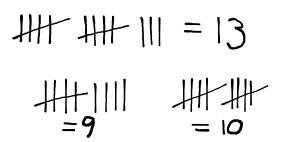
\includegraphics[width=4cm]{strecktal.png}
	\caption{Tecknen i ett enkelt teckenv�rdessystem.}
	\label{fig:Strecktal}
\end{figure}

Det romerska systemet �r en modifiering av detta system.
Tecknen och deras betydelse i det romerska talsystemet ges i
\tblref{tbl:RomerskaSiffror}.

\begin{table}[h]
	\caption{De romerska siffrorna.}
	\begin{tabular}{ccccccc}
		\hline\hline
		I & V & X & L & C & D & M \\
		1 & 5 & 10 & 50 & 100 & 500 & 1000 \\
		\hline\hline
	\end{tabular}
	\label{tbl:RomerskaSiffror}
\end{table}

Det romerska talsystemt fungerar n�stan p� samma s�tt som ett
tecken\-v�rdes\-system.
Den v�sentliga skillnaden �r att i teckenv�rdessystemet summeras alla tecknens
v�rden medan det i det romerska systemet �ven finns subtraktion.
I det romerska systemet subtraheras ett tecken av l�gre v�rde som st�r f�re ett
tecken med h�gre v�rde.
Exempelvis, IV ger \(4\) eftersom att en etta st�r f�re en femma.
VI ger d�remot \(6\) eftersom att tecknens v�rde summeras.
Talen 1-10 ges i \tblref{tbl:RomerskaTal} och n�gra andra st�rre tal finns i
\tblref{tbl:RomerskaTal2}.

\begin{table}[h]
	\caption{Talen 1-10 i det decimala och det romerska talsystemen.}
	\begin{tabular}{l|llllllllll}
		\hline\hline
		Decimala talsystemet & 1 & 2 & 3 & 4 & 5 & 6 & 7 & 8 & 9 & 10 \\
		Romerska talsystemt & I & II & III & IV & V &
			VI & VII & VIII & IX & X \\
		\hline\hline
	\end{tabular}
	\label{tbl:RomerskaTal}
\end{table}

\begin{table}[t]
	\begin{tabular}{lll}
		\hline\hline
		\(2011\) & MMXI & \(1000+1000+10+1\) \\
		\(1999\) & MCMXCIX & \(1000+(1000-100)+(100-10)+(10-1)\) \\
		\(1998\) & MCMXCVIII & \(1000+(1000-100)+(100-10)+5+1+1+1\) \\
		\(587\) & DLXXXVII & \(500+50+10+10+10+5+1+1\) \\
		\(487\) & CDLXXXVII & \((500-100)+50+10+10+10+5+1+1\) \\
		\hline\hline\\
	\end{tabular}
	\caption{N�gra tal skrivna med det romerska talsystemet.}
	\label{tbl:RomerskaTal2}
\end{table}

Som kan ses i \tblref{tbl:RomerskaTal2} �r det efterstr�vansv�rt att s� f�
tecken som m�jligt anv�nds vid subtraktion.
Exempelvis kan t�nkas att \(487\) �r \(500\) minus \(13\) och d�rf�r skulle
kunna skrivas som XIIID.
Det blir dock enklare att se om man ist�llet anv�nder C, eller \(100\), f�r
subtraktionen av D, eller \(500\), och sedan l�gger till tecknen f�r \(87\)
som vanligt.

\begin{exercise}\label{xrc:RaknaMedRomerskaTal}
	Unders�k och diskutera hur enkelt det �r att r�kna med och
	representera tal med det romerska talsystemet.
\end{exercise}
\begin{exercise}
	Med utg�ngspunkt i f�reg�ende �vning, hur tror du att romarna bidragit till
	matematikhistorien?
\end{exercise}
\begin{exercise}
	Hur �r det med talet noll och negativa tal i det romerska talsystemet?
\end{exercise}



%%%%%%%%%%%%%%%%%%%%%%%%%%%%%%%%%%%%%%%%%
% POSITIONSSYSTEM
%%%%%%%%%%%%%%%%%%%%%%%%%%%%%%%%%%%%%%%%%
\section{Positionssystem}
\index{positionssystem}\index{talsystem!positionssystem}
\label{sec:Positionssystem}
\noindent
\lettrine{S}{om n�mnts tidigare} inneb�r ett positionssystem att samma tecken
har olika betydelse eller v�rde beroende p� vilken position tecknet innehar.
Systemet har en \emph{talbas}.
Det decimala talsystemet har basen \(10\) och varje position motsvarar en
unik \(10\)-potens.
Siffran p� denna position ger koefficienten f�r denna potens.

\begin{example}\label{ex:DecimaltPosistionssystem}
	Det decimala talsystemet har basen \(10\).
	Talet etthundratjugotre representeras i detta system som \(123\).
	Vi har d�
	\[1\cdot10^2 + 2\cdot10^1 + 3\cdot10^0 = 100 + 20 + 3 = 123.\]
\end{example}
\begin{example}\label{ex:BinartPositionssystem}
	Det bin�ra talsystemet har basen \(2\).
	S�ledes representeras talet etthundratjugotre som \(1111011\).
	Vi har d�
	\[1\cdot2^6 + 1\cdot2^5 + 1\cdot 2^4 + 1\cdot2^3 + 0\cdot2^2 +
	1\cdot2^1 + 1\cdot2^0 = 123.\]
\end{example}
\begin{example}
	Om ett positionssystem har basen \(b\) anv�nds d� \(b\) antal siffror,
	dessa har v�rdena \(0, 1, 2, \ldots, b-1\).
	F�r att representera ett tal anv�nds summor av \(b\)-potenser d�r siffrans
	position avg�r exponenten.
	Siffrans v�rde avg�r koefficienten f�r, det vill s�ga hur m�nga av, den
	specifika \(b\)-potensen som ska adderas.
	Det vill s�ga talet vars v�rde ber�knas som
	\[
		d_1b^{n-1} + d_2b^{n-1} + \cdots + d_{n-1}b^1 + d_nb^0
	\]
	representeras som \(d_1d_2\cdots d_n\) i basen \(b\).
\end{example}

Det finns �ven andra talsystem, exempelvis babyloniernas
sexagesimala positionssystem\index{talsystem!babylonskt}
\index{talsystem!sexagesimalt} som hade basen \(60\).
Sp�r av detta kan vi idag se i hur vi r�knar tid, att en minut har 60
sekunder och en timme har 60 minuter.
Vi anv�nder dock inte 60 olika tecken f�r att representera v�ra sekunder och
minuter utan tar ist�llet hj�lp av det decimala talsystemet.
Det babylonska sexagesimalsystemet �r det �ldsta k�nda anv�ndandet av ett
positionssystem och h�rstammar fr�n Babylonien\footnote{Babylonien l�g i
s�dra delen av Mesopotamien, ungef�r i dagens Irak.} omkring 3100 f.Kr.
\nocite{Kline1990mtf1}

Kan d� alla naturliga tal verkligen representeras med en godtycklig bas p�
detta s�tt?
F�ljande sats visar att s�dant �r fallet.
\begin{theorem}\label{thm:PositionssystemAllaUnika}
	L�t \(b>1\) vara ett naturligt tal st�rre �n ett.
	F�r varje naturligt tal \(x\in\N\) existerar ett naturligt tal \(n>0\)
	strikt st�rre �n noll och naturliga tal \(d_i<b\), d�r \(1\leq i\leq n\),
	strikt mindre �n \(b\) s�dana att \(x\) kan skrivas som
	\begin{equation*}
		x = d_1b^{n-1} + d_2b^{n-2} + \cdots + d_{n-1}b^1 + d_nb^0.
	\end{equation*}
	Denna presentation �r unik upp till ordningen av termerna.
\end{theorem}
F�r att kunna bevisa detta beh�ver vi f�rst f�ljande lemma.
\begin{lemma}
	\label{lem:NollEndastOmLika}
	L�t \(b>0\) vara ett naturligt tal st�rre �n noll, \(m\) och \(n\)
	naturliga tal och \(c=c_1b^{n-1}+c_2b^{n-2}+\cdots+c_{n-1}b+c_n\), d�r
	\(0<c_1<b\) och \(0\leq c_i<b\) f�r \(i=2,3,\ldots,n\), och
	\(d=d_1b^{m-1}+d_2b^{m-2}+\cdots+d_{m-1}b+d_m\), d�r \(0<d_1<b\) och \(0\leq
	d_j<b\) f�r \(j=2,3,\ldots,m\).
	D� g�ller att \(c-d=0\) endast om \(n=m\) och \(c_i=d_i\) f�r
	\(i=1,2,3,\ldots,n\).
\end{lemma}
\begin{proof}
	L�t oss anta att \(n=m+k\) f�r n�got naturligt tal \(k\).
	Vi har d� att
	\begin{equation*}
		c-d=c_1b^{n-1}+\cdots+c_{k-1}b^{n-k+1}+(c_k-d_0)b^m+\cdots+(c_n-d_m) =
		0.
	\end{equation*}
	Men \(c_1b^{n-1}\neq 0\) och d� m�ste \(n=m\).

	D� har vi att
	\begin{equation*}
		c-d = (c_1-d_1)b^{n-1}+\cdots+(c_{n-1}-d_{n-1})b+(c_n-d_n) = 0.
	\end{equation*}
	L�t oss anta att \(c_n-d_n\neq 0\), om inte delar vi med \(b\) tills att vi
	f�r en nollskild term utan en faktor \(b\).
	D� f�r vi att
	\begin{equation}
		\label{eq:NollEndastOmLika}
		(c_0-d_0)b^n+\cdots+(c_{n-1}-d_{n-1})b = -(c_n-d_n).
	\end{equation}
	Eftersom att v�nsterledet i \eqref{eq:NollEndastOmLika} �r delbart med
	\(b\) m�ste �ven h�gerledet vara detta eftersom att de �r lika.
	Men eftersom att \(c_i<b\) och \(d_i<b\) har vi att
	\(-b<c_i-d_i<b\) f�r \(i=0,1,2,\ldots,n\).
	D� �r \(-(c_n-d_n)\) delbar med \(b\) endast om \(-(c_n-d_n)=0\), vilket
	�r en mots�gelse.
	D� m�ste alla termer \(c_i-d_i=0\) f�r \(i=1,2,3,\ldots,n\).
\end{proof}

Nu �r vi redo att visa satsen.
\begin{proof}[Bevis \thmref{thm:PositionssystemAllaUnika}]
	Vi b�rjar med att visa att summan existerar.
	Om vi delar \(x\) med \(b\) f�r vi en kvot \(q_1\) och en restterm
	\(r_1\) s�dana att \(x=q_1b+r_1\) och \(0\leq r_1<b\).
	Om vi p� samma vis delar \(q_1\) med \(b\) f�r vi en kvot \(q_2\) och en
	restterm \(r_2\) s�dana att \(q_1=q_2b+r_2\) och \(0\leq r_2 < b\).
	Upprepas detta f�rfarande f�r vi att \(q_i=q_{i+1}b+r_{i+1}\), \(i\in\N\).
	Fr�n \xrcref{xrc:KvotenMindre} har vi att \(q_{i+1}<q_i\) eftersom att
	\(b>1\).
	Vi f�r d� fr�n v�lordningsprincipen f�r de naturliga talen att \(q_n=0\)
	f�r n�got \(n\in\N\).
	Vi nu s�tter ihop dessa resultat enligt f�ljande id�.
	Vi hade f�rst att \(x=q_1b+r_1\), men \(q_1=q_2b+r_2\) och f�ljaktligen �r
	\[x=(q_2b+r_2)b+r_1.\]
	Eftersom att \(q_i=q_{i+1}b+r_{i+1}\) f�r vi att
	\begin{align*}
		x &= ((((q_nb+r_n)b+r_{n-1})b+\cdots+r_3)b+r_2)b+r_1 \\
		 &= r_nb^{n-1}+r_{n-1}b^{n-2}+\cdots+r_3b^2+r_2b^1+r_1b^0.
	\end{align*}
	Om vi l�ter \(d_1=r_n, d_2=r_{n-1}, \ldots, d_{n-1}=r_2, d_n=r_1\) ser vi
	att vi f�r en summa p� korrekt form.

	Antag att det f�r ett naturligt tal \(x\) finns tv� olika representationer
	\(c_1c_2\cdots c_n\) och \(d_1d_2\cdots d_m\), b�da med basen \(b\).
	Detta inneb�r att
	\begin{equation*}
		c_1b^{n-1}+c_2b^{n-2}+\cdots+c_nb^0 =
		x =
		d_1b^{m-1}+d_2b^{m-2}+\cdots+d_mb^0.
	\end{equation*}
	D� m�ste
	\begin{equation*}
		c_1b^{n-1}+c_2b^{n-2}+\cdots+c_n - d_1b^{m-1}+d_2b^{m-2}+\cdots+d_m =
		0,
	\end{equation*}
	men enligt \lemref{lem:NollEndastOmLika} kan detta ej vara sant och vi har
	en mots�gelse.
	D� m�ste det vara samma representation.

%	Antag att det �ven finns ett tal \(y\neq x\) skilt fr�n \(x\) men med
%	samma representation.
%	D� har vi att
%	\begin{equation*}
%		y = r_nb^{n-1}+\cdots+r_2b^1+r_1.
%	\end{equation*}
%	Men
%	\begin{equation*}
%		x = r_nb^{n-1}+\cdots+r_2b^1+r_1 = y,
%	\end{equation*}
%	vilket �r en mots�gelse eftersom att vi antagit \(x\neq y\).
%	Allts� kan inget s�dant tal \(y\) existera och representationen m�ste
%	d�rf�r vara unik.
\end{proof}

\begin{exercise}
	Diskutera inneb�rden av denna sats och dess bevis.
\end{exercise}

\begin{example}
	Det kan nu vara av intresse med ett exempel d�r representationen ej �r unik.
	Ett tydligt exempel �r det romerska talsystemet d�r \(99\) skulle kunna
	representeras av b�de IC och XCIX.
	Representationen f�r tal i det romerska systemet �r d�rmed inte unik.
\end{example}

Eftersom att vi enligt \thmref{thm:PositionssystemAllaUnika} kan representera
alla naturliga tal i en godtycklig bas \(b>1\) st�rre �n ett och att denna
representation �r unik kan vi med s�kerhet definiera ett positionssystem enligt
f�ljande.
\begin{definition}[Positionssystem\footnote{\emph{Eng.} positional system,
	place-value system}]
	\index{talsystem!positionssystem}\index{positionssystem}
	\index{talbas}\index{positionssystem!talbas}
	\index{positionsv�rdesystem|see{positionssystem}}
	\label{def:Positionssystem}
	Ett \emph{positionssystem}, eller positionsv�rdesystem, har en
	\emph{talbas} \(b \in \N \setminus \{0,1\}\),
	siffrorna \(S=\{s\in\N : s<b\}\) och representerar ett tal \(x\in\N\) som
	\(d_1d_2\cdots d_n\), d�r \(d_i \in S\) �r siffran p� position \(i\), och
	\begin{equation}
		\nonumber
		x = d_1b^{n-1} + d_2b^{n-2} + \ldots + d_{n-1}b^1 + d_nb^0.
	\end{equation}
\end{definition}

\begin{example}\label{ex:DecimalaTalsystemet}
	Det decimala talsystemet har basen \(b=10\) och anv�nder siffrorna
	\(S=\{0,1,2,3,4,5,6,7,8,9\}\).
\end{example}
\begin{example}\label{ex:BinaraTalsystemet}
	Det bin�ra talsystemet har basen \(b=2\) och anv�nder siffrorna
	\(S=\{0,1\}\).
\end{example}
\begin{example}\label{ex:HexadecimalaTalsystemet}
	Det hexadecimala talsystemet har basen \(b=16\).
	N�r ett talsystem har basen \(b>10\) anv�nds vanligtvis bokst�ver fr�n
	alfabetet som siffror f�r v�rdena \(10\), \(11\) och s� vidare.
	Det hexadecimala talsystemet anv�nder vanligtvis
	siffrorna \[S=\{0,1,2,3,4,5,6,7,8,9,A,B,C,D,E,F\},\] d�r \(A=10\),
	\(B=11\), \dots, \(F=15\).
\end{example}

F�r att kunna urskilja vilken talbas ett tal representeras med brukar basen
anges som ett subskript.
Exempelvis talet \(123\) skrivet med det decimala systemet anges som
\(123_{10}\).
Det blir d� l�ttare att f�rst� \(123_{10} = 1111011_2\) som betyder att \(123\)
i bas 10 skrivs som \(1111011\) i bas 2.
Vanligtvis, n�r basen �r sj�lvklar, brukar den utel�mnas.
I de f�rsta 9 �ren i grundskolan �r det uteslutande det decimala talsystemet
som anv�nds och det har d�rf�r aldrig varit n�dv�ndigt att d�r specificera att
basen varit 10.

\begin{exercise}\label{xrc:GiltigaTalbaser}
	Enligt \defref{def:Positionssystem} anv�nds inte talen \(0\) och \(1\)
	som baser, f�rs�k att f�rklara varf�r.
\end{exercise}
\begin{exercise}\label{xrc:RationelltPositionssystem}
	Vidareutveckla \defref{def:Positionssystem} till att �ven
	omfatta rationella tal.
\end{exercise}
\begin{exercise}\label{xrc:KomplettRationelltPositionssystem}
	Visa att alla rationella tal kan representeras med en godtycklig bas
	\(1<b\in\N\) enligt den nya definitionen fr�n
	\xrcref{xrc:RationelltPositionssystem}.
\end{exercise}
\begin{exercise}\label{xrc:Decimalfoljder}
	Det rationella talet \(\frac{1}{3} = 0.333\ldots\) skrivs som en o�ndlig
	decimalutveckling i bas \(10\).
	�r det s� i alla baser \(1<b\in\N\)?
\end{exercise}
\begin{exercise}\label{xrc:Basbyte}
	F�rs�k att formulera en metod f�r att byta talbas f�r ett tal.
\end{exercise}


%%%%%%%%%%%%%%%%%%%%%%%%%%%%%%%%%%%%%%%%%%%%%%%%%%%%%%%%%%%%%%
% BYTE AV TALBAS
%%%%%%%%%%%%%%%%%%%%%%%%%%%%%%%%%%%%%%%%%%%%%%%%%%%%%%%%%%%%%%
\section{Byte av talbas}
\noindent
\lettrine{E}{ftersom att} \thmref{thm:PositionssystemAllaUnika} s�ger att alla
naturliga tal kan representeras i alla baser inneb�r detta att samma tal har
en unik representation i varje bas.
Det kan d� vara intressant att se ett tals olika representationer i olika
baser.
Hur detta basbyte g�r till och att det fungerar framg�r av beviset f�r satsen.
Metoden illustreras h�r med nedan givna exempel.
\begin{example}
	Talet \(123_{10} = 1111011_2\), detta finner vi genom f�ljande:
	\begin{align*}
		123 &= 61\cdot 2 + 1 \\
		61 &= 30\cdot 2 + 1 \\
		30 &= 15\cdot 2 + 0 \\
		15 &= 7\cdot 2 + 1 \\
		7 &= 3\cdot 2 + 1 \\
		3 &= 1\cdot 2 + 1 \\
		1 &= 0\cdot 2 + 1
	\end{align*}
	D� f�r vi
	\begin{multline}
%		(((((((0+1)\cdot2 + 1)\cdot2 + 1)\cdot2 + 1)\cdot2 + 1) + 0)\cdot2 + 1)
%			\cdot2 + 1 \\
		1 + 2\cdot (1 + 2\cdot (0 + 2\cdot (1 + 2\cdot (1 + 2\cdot (1 + 2\cdot
			(1 + 0)))))) \\
		= 1\cdot 2^6 + 1\cdot 2^5 + 1\cdot 2^4 + 1\cdot^3 + 0\cdot 2^2 +
			1\cdot 2^1 + 1\cdot 2^0 \\
		= 1111011_2 = 123_{10}.
	\end{multline}
\end{example}
\begin{example}
	Talet \(123_{10} = 7B_{16}\), detta finner vi genom f�ljande:
	\begin{align*}
		123 &= 7\cdot16 + 11 \\
		7 &= 0\cdot16 + 7
	\end{align*}
	S�ledes f�r vi siffrorna \(7\) och \(B\) samt att
	\begin{equation*}
		(0+7)\cdot16 + 11 = 7\cdot16^1 + 11\cdot16^0 = 7B_{16} = 123_{10}.
	\end{equation*}
	Detta betyder att \(7B_{16} = 123_{10}\) och d�rf�r �r \(7B\) hexadecimalt
	samma tal som 123 �r decimalt.
\end{example}

\begin{exercise}
	Vilket tal representerar \(123\) n�r det hexadecimala talsystemet anv�nds?
	Det vill s�ga, hur representeras \(123_{16}\) med basen 10?
\end{exercise}

\begin{exercise}\label{xrc:TalbasDatavetenskap}
	Inom datateknik �r baserna \(2=2^1\), \(8=2^3\) och \(16=2^4\) v�ldigt
	popul�ra, men bas \(10=2\cdot5\) �r d�remot inte lika popul�r.
	Datorns interna representation av tal sker i form av \emph{bitar} som kan
	anta v�rdena \emph{p�} och \emph{av}, eller \(1\) och \(0\).
	Detta motsvarar precis det bin�ra talsystemet, det vill s�ga basen
	\(2=2^1\), detta f�rklarar basens popularitet.
	F�rs�k att f�rklara varf�r baserna \(8=2^3\) och \(16=2^4\) �r popul�ra,
	medan bas \(10=2\cdot5\) inte �r det.
\end{exercise}



%%%%%%%%%%%%%%%%%%%%%%%%%%%%%%%%%%%%%%%%%%%%%%%%%%%%%%%%%%%%%%
% EN ADDITIONSALGORITM
%%%%%%%%%%%%%%%%%%%%%%%%%%%%%%%%%%%%%%%%%%%%%%%%%%%%%%%%%%%%%%
\section{En additionsalgoritm}
\noindent
\lettrine{P}{ositionens betydelse} f�r siffrornas v�rde i positionssystemet g�r
att tal representerade i detta talsystem blir v�ldigt enkla att r�kna med.
Vi ska i detta avsnitt unders�ka varf�r.

Vi inleder f�rst med en illustration av algoritmen genom f�ljande exempel.
\begin{example}
	Vi vill addera talen \(123_{10}\) och \(253_{10}\) i basen \(10\).
	Vi skriver dem d� ovanf�r varandra och f�r d� steg \verb'a)' nedan.
	\begin{verbatim}
     a)   1 2 3   b)   1 2 3  c)   1 2 3  d)   1 2 3
        + 2 5 3      + 2 5 3     + 2 5 3     + 2 5 3
        -------      -------     -------     -------
                           6         7 6       3 7 6
	\end{verbatim}
	Vi forts�tter genom att addera siffrorna i den sista kolumnen, det vill
	s�ga entalen.
	Vi f�r d� \(3\) och \(3\), och totalt har vi \(6\).
	Detta tal skriver vi under raden och hamnar d� i steg \verb'b)'.
	Vi forts�tter p� samma s�tt i stegen \verb'c)' och \verb'd)'.
	I steg \verb'c)' adderar vi tiotalen och i steg \verb'd)' adderar vi
	hundratalen.
	Summan av de tv� talen �r talet som st�r under raden, det vill s�ga
	\(123+253=376\).
\end{example}
\begin{example}\label{ex:AdderaMedRest}
	Vi vill nu addera talen \(123_{10}\) och \(999_{10}\), fortfarande i basen
	\(10\).
	Vi g�r d� som ovan och f�r steg \verb'a)' nedan.
	\begin{verbatim}
                         1         1 1       1 1 1       1 1 1
     a)   1 2 3   b)   1 2 3  c)   1 2 3  d)   1 2 3  e)   1 2 3
        + 9 9 9      + 9 9 9     + 9 9 9     + 9 9 9     + 9 9 9
        -------      -------     -------     -------     -------
                           2         2 2       1 2 2     1 1 2 2
	\end{verbatim}
	Vi forts�tter genom att addera siffrorna i den sista kolumnen, det vill
	s�ga entalen \(3\) och \(9\), och f�r d� \(12\).
	Eftersom att vi f�r \(12\) ental inneb�r detta att vi f�r ett tiotal och
	tv� ental.
	Tiotal adderas tillsammans med tiotal och vi skriver \(1\) ovanf�r kolumnen
	med tiotal.
	Vi hamnar d� i steg \verb'b)'.
	I steg \verb'c)' adderar vi kolumnen med talen \(1, 2\) och \(9\), det vill
	s�ga alla tiotal.
	Vi f�r �ter \(12\) och g�r som i steg \verb'b)' eftersom att \(12\) tiotal
	inneb�r att vi har ett hundratal och tv� tiotal.
	I steg \verb'c)' n�r vi adderar \(1,1\) och \(9\) f�r vi \(11\).
	Detta inneb�r att vi f�r ett hundratal och ett tusental.
	Eftersom att det inte fanns n�gra tusental i de b�da termerna skriver vi
	tusentalet ovanf�r den tomma kolumnen till v�nster, detta visas i steg
	\verb'd)'.
	I steg \verb'e)' adderar vi \(1,0\) och \(0\) och f�r \(1\) som skrivs
	under raden.
	D� f�r vi att \(123+999=1122\).
\end{example}
\begin{remark}
	Notera att tiotalet ges av kvoten vid heltalsdivision med basen som
	n�mnare, dessutom ges entalet av resten vid denna heltalsdivision.
%	Notera att entalet ges av resten vid heltalsdivision med basen som n�mnare
%	och tiotalet ges av heltalskvoten. %vid denna heltalsdivision.
\end{remark}

Vi vill nu titta p� det generella fallet med en godtycklig bas \(b>1\).
N�r vi ovan adderar kolumnerna kan vi f� ett en- eller tv�siffrigt tal som
resultat.
Till exempel n�r vi i \exref{ex:AdderaMedRest} steg \verb'b)' adderar \(3\)
och \(9\) f�r vi det tv�siffriga talet \(12\).
Om \(b>1\) �r basen i ett talsystem, \(s<b\) och \(t<b\) �r tv� siffror i detta
talsystem.
D� �r summan \(0\leq s+t\leq 2(b-1)\).
Om summan \(s+t\) �r strikt mindre �n \(b\) f�ljer det av
\thmref{thm:PositionssystemAllaUnika} att summan �r ensiffrig.
F�ljande lemma fastst�ller att om summan \(s+t\) �r st�rre �n \(b\) och mindre
�n \(2(b-1)\) d� �r summan exakt tv�siffrig.
\begin{lemma}\label{lem:AdditionSiffror}
	Ett naturligt tal \(x\) i intervallet \(b \leq x \leq 2(b-1)\) kan skrivas
	som en summa \(x = d_1b^1 + d_2b^0\),
	d�r \(1 \leq d_1 \leq b-1\) och \(0 \leq d_2 \leq b-1\).
\end{lemma}
\begin{proof}
	Det �r klart fr�n \thmref{thm:PositionssystemAllaUnika} att \(x\) kan
	skrivas som en summa p� formen \(d_1b^{n-1}+\cdots+d_nb^0\) och att denna
	�r unik.
	Det som �terst�r att visa �r att den best�r av enbart tv� termer, det vill
	s�ga att \(n=2\).

	Om vi tittar p� fallet \(x=b\) f�r vi vid heltalsdivision kvoten \(x/b = 1\)
	och resttermen \(0\).
	Det vill s�ga, vi har \(d_1=1\), \(d_2=0\) och s�ledes \(x=1\cdot b+0\).
	D� m�ste vi ha minst tv� termer.

	Om vi tittar p� fallet \(x=2(b-1)\) ser vi att \(2(b-1)=b+(b-2)\).
	Heltalsdivisionen \(x/b\) ger d� kvoten \(b/b=1\) och resttermen \(b-2\).
	Vi har s�ledes \(d_1=1\), \(d_2=b-2\) och f�ljaktligen
	\(x=1\cdot b+(b-2)\).

	D� har vi exakt tv� termer.
\end{proof}

\begin{exercise}
	Diskutera inneb�rden av detta lemma och dess bevis.
\end{exercise}

Innan vi g�r vidare till satsen som visar att denna additionsmetod fungerar
m�ste vi ha lite notation f�r att underl�tta formuleringarna.
L�t \(q_b\) vara en funktion s�dan att den ger kvoten vid heltalsdivisionen
\(t/b\) och beteckna denna som \(q_b(t)\).
L�t ocks� \(r_b\) vara en funktion s�dan att den ger resten vid
heltalsdivisionen \(t/b\) och beteckna denna som \(r_b(t)\).
D� har vi att \(t=q_b(t)\cdot b+r_b(t)\).
\begin{example}
	Vi har att \(q_5(7)=7/5=1\) och \(r_5(7)=7-q_5(7)\cdot 5=2\).
\end{example}
\begin{example}
	Vi har att \(q_{10}(7)=7/10=0\) och \(r_{10}(7)=7-q_{10}(7)\cdot 10=7\).
\end{example}

F�ljande sats visar att denna additionsmetod fungerar f�r godtyckligt l�nga tal
\(x=x_1x_2\cdots x_n\) och \(y=y_1y_2\cdots y_m\) representerade i samma talbas
\(b>1\).
\begin{theorem}[Additionsalgoritm]
	L�t \(x=x_1x_2\cdots x_n\) och \(y=y_1y_2\cdots y_m\) vara tv� tal
	representerade i ett positionssystem med basen \(b>1\),
	\(x_i\) och \(y_i\) vara identiskt noll f�r \(i<1\) och \(N=\max\{n,m\}\).
	L�t ocks� \(q_b(t)=t/b\) vara kvoten och \(r_b(t)\) vara resten vid
	heltalsdivisionen \(t/b\).
	Summan \(x+y\) kan d� f�s genom 
	\begin{multline}\label{eq:AdditionsEkvation}
		x+y= q_b(x_{n-N}+y_{m-N})b^N + \\
		\left(r_b(x_{n-N}+y_{m-N})+q_b(x_{n-N+1}+y_{m-N+1})\right)b^{N-1} +\\
		\left(r_b(x_{n-N+1}+y_{m-N+1})+q_b(x_{n-N+2}+y_{m-N+2})\right)b^{N-2}
			+ \\
		\cdots + \left(r_b(x_{n-1}+y_{m-1})+q_b(x_n+y_m)\right)b^1 +
		r_b(x_n+y_{m})b^0.
	\end{multline}
\end{theorem}
\begin{proof}
	L�t oss f�rst antaga att \(n=m+k\).
	Om vi tittar p� \(x=x_1b^{n-1}+x_2b^{n-2}+\cdots+x_nb^0\) och
	\(y=y_1b^{m-1}+y_2b^{m-2}+\cdots+y_mb^0\) f�r vi att
	\begin{align*}
		x+y=&x_1b^{n-1}+\cdots+x_{k-1}b^{n-k+1}+(x_k+y_1)b^m+\\
		&(x_{k+1}+y_2)b^{m-1}+\cdots+(x_{n-1}+y_{m-1})b^1+(x_n+y_m)b^0
	\end{align*}
	Vi forts�tter med att titta p� en av termerna \((x_{i+k}+y_i)b^{n-k-i}\)
	och vi ser att \(0\leq x_{i+k}+y_i\leq b-2\).
	Vi har fr�n \lemref{lem:AdditionSiffror} att om \(b\leq x_{i+k}+y_i\leq
	2(b-1)\) �r \(x_{i+k}+y_i = d_1b+d_2\) med \(1\leq d_1<b\) och \(0\leq
	d_2<b\) och \(x_{i+k}+y_i = d < b\) annars.

	Vi tittar p� det f�rsta fallet.
	Vi f�r d� att
	\begin{align*}
		(x_{i+k}+y_i)b^{n-k-i} &= (d_1b+d_2)b^{n-k-i}
			= d_1b^{n-k-i+1}+d_2b^{n-k-i}.
	\end{align*}
	Vi har att \(q_b(d_1b+d_2)=d_1\) och att \(r_b(d_1b+d_2)=d_2\) och s�ledes
	att
	\begin{equation*}
		(x_{i+k}+y_i)b^{n-k-i} = q_b(x_{i+k}+y_i)b^{n-k-i+1} +
		r_b(x_{i+k}+y_i)b^{n-k-i}.
	\end{equation*}
	Om \(x_{i+k}+y_i<b\) har vi att \(q_b(x_{i+k}+y_i)=0\) och
	\(r_b(x_{i+k}+y_i)=x_{i+k}+y_i\) och d� f�r vi �ven med det andra
	fallet.

	Vi ser i \eqref{eq:AdditionsEkvation} att b�da dessa termer finns med.
	\(q_b(x_{i+k}+y_i)\) finns med som en del i \(b^{n-k-i+1}\)-potensen och
	\(r_b(x_{i+k}+y_i)\) finns med som en del i \(b^{n-k-i}\)-potensen.

	Vi kan s�ledes konstatera att likheten i \eqref{eq:AdditionsEkvation} �r
	korrekt.
\end{proof}
\begin{exercise}
	Diskutera inneb�rden av denna sats och dess bevis.
\end{exercise}

Med detta har vi visat att additionsmetoden fungerar f�r en godtycklig bas
\(b>1\) i ett positionssystem.
Alla \(q_b\)-termerna motsvarar tiotalet som skrivs ovanf�r v�nstervarande
kolumn om summan blir f�r stor.
Om summan inte blir f�r stor blir \(q_b\)-termen noll.
Alla \(r_b\)-termerna motsvarar entalet som alltid skrivs under strecket.

\begin{exercise}\label{xrc:MultiplikationsAlgoritm}
	Unders�k om den v�lk�nda multiplikationsalgoritmen, som elever l�r sig i den
	svenska grundskolan, �ven den fungerar f�r alla baser \(1<b\in\N\).
\end{exercise}
\begin{exercise}
	Bevisa ditt resultat fr�n \xrcref{xrc:MultiplikationsAlgoritm}.
\end{exercise}


\backmatter
\ifdraft{
	\singlespacing
}{}
%\bibliographystyle{kthnat}
\bibliographystyle{sweplnat}
\bibliography{../thesis/thesis}

\listoffigures
\listoftables
\clearpage
\printindex
\clearpage


% appendices
\appendix
\ifdraft{
	\doublespacing
}{}
%\chapter{Kursplanering}\label{app:Kursplanering}
\nocite{ibmath}
\noindent
\lettrine{K}{ursen Matematik 1c}
% Kursen Matematik 1c
�r enligt �mnesplanen 100 po�ng, det vill s�ga den ska ges 100 lektionstimmar.
Dessa lektionstimmar ska f�rdelas p� de fem huvudomr�den som ges under rubriken
\emph{Centralt inneh�ll} i �mnesplanen: 
\begin{itemize}
	\item Taluppfattning, aritmetik och algebra,
	\item Geometri,
	\item Samband och f�r�ndring,
	\item Sannolikhet och statistik, samt
	\item Probleml�sning.
\end{itemize}

I planeringen given nedan avser tids�tg�ngen l�rargenomg�ngar, till exempel
tid n�r l�raren g�r igenom inneh�ll vid tavlan.
Denna tid innefattar inte elevers egna arbete, redovisningar av uppgifter,
klassrumsdiskussioner etcetera.

Avsnittet \emph{Probleml�sning}, som inneh�ller punkterna
\begin{itemize}
	\item Strategier f�r matematisk probleml�sning inklusive anv�ndning av
		digitala medier och verktyg,
	\item Matematiska problem av betydelse f�r privatekonomi, samh�llsliv och
		till�mpningar i andra �mnen, och
	\item Matematiska problem med anknytning till matematikens kulturhistoria,
\end{itemize}
kan med f�rdel inkluderas i undervisningen som tar upp �vriga omr�den och
beh�ver s�ledes inte behandlas specifikt.

Inledande i kursen b�r vara grundl�ggande logik\footnote{Fr�n omr�det
\emph{Geometri} har vi punkten ''Matematisk argumentation ned hj�lp av
grundl�ggande logik inklusive implikation och ekvivalens samt j�mf�relser med
hur man argumenterar i vardagliga sammanhang och inom naturvetenskapliga
�mnen''.}, begreppen definition och axiom samt sats och bevis\footnote{Fr�n
omr�det \emph{Geometri} har vi punkten ''Illustration av begreppen definition,
sats och bevis, till exempel med Pythagoras sats och triangelns vinkelsumma''.}.
Detta eftersom att dessa fundamentala begrepp �r det som bygger upp
matematiken.
D�refter kan grundl�ggande m�ngdl�ra g�s igenom, med axiom och grundl�ggande
satser, och konstruktionen av de naturliga talen kan visas f�r att visa hur
matematiken fundamentalt �r uppbyggd.
F�r detaljer se \tblref{tbl:inledning}.

\begin{table}[h]
	\caption{Planering f�r inledningen.}
	\begin{tabular}{ll}
		Inneh�ll & Tids�tg�ng (timmar) \\
		\hline\hline
		Logik, definition, sats och bevis. & 2 \\
		\hline
		M�ngder. & 1 \\
		\hline
		M�ngden av naturliga tal. & 1 \\
		\hline\hline
		& 4 \\
		\hline\hline\\
	\end{tabular}
	\label{tbl:inledning}
\end{table}

D�refter f�ljer l�mpligen avsnittet \emph{Taluppfattning, aritmetik
och algebra} eftersom att taluppfattning, aritmetik och algebra �r n�dv�ndiga
f�r vidare studier av matematiken, och allts� n�dv�ndiga f�r resten av kursen,
samt att det �r naturligt att studera heltalen efter de naturliga talen.
F�r detaljer se \tblref{tbl:talteori}.
%Eftersom att avsnittet har fem punkter b�r \emph{25 timmar} avs�ttas f�r hela
%detta omr�de.

\begin{table}[h]
	\caption{Planering f�r avsnittet \emph{Taluppfattning, aritmetik och
		algebra}.}
	\begin{tabular}{ll}
		%\textbf{Inneh�ll} & \textbf{Tids�tg�ng (timmar)} \\
		Inneh�ll & Tids�tg�ng (timmar) \\
		\hline\hline
		Generalisering av aritmetikens r�kneregler till att\\
			hantera algebraiska uttryck. & 2 \\
		\hline
		Egenskaper hos m�ngden heltal, olika talbaser samt\\
			begreppen primtal och delbarhet. & 5 \\
		\hline
		Egenskaper hos m�ngderna rationella tal, irrationella\\
			tal och reella tal. & 5 \\
		\hline
		Begreppet linj�r olikhet. & 1 \\
		\hline
		Algebraiska och grafiska metoder f�r att l�sa linj�ra\\
			ekvationer, olikheter och potensekvationer. & 5 \\
		\hline
		Metoder f�r ber�kningar inom vardagslivet och\\
			karakt�rs�mnena med reella tal skrivna p� olika\\
			former, inklusive potenser med reella exponenter\\
			samt strategier f�r anv�ndning av digitala verktyg.
			& * \\
		\hline\hline
		& 21 \\
		\hline\hline\\
	\end{tabular}
	\label{tbl:talteori}
\end{table}

Efter egenskaperna hos heltal, rationella och irrationella tal och algebra kan
funktionsbegreppet introduceras.
Funktionsbegreppet �r ett centralt begrepp inom all matematik och b�r g�s
igenom tidigt i kursen f�r att kunna anv�ndas senare, exempelvis n�r
de trigonometriska funktionerna och logaritmfunktionen introduceras.
F�r detaljer se \tblref{tbl:funktioner}.

\begin{table}[h]
%	\caption{Planering f�r avsnittet \emph{Samband och f�r�ndring}, del 1.}
	\caption{Planering f�r avsnittet \emph{Samband och f�r�ndring}.}
	\begin{tabular}{ll}
		Inneh�ll & Tids�tg�ng (timmar) \\
		\hline\hline
		Begreppen funktion, definitions- och v�rdem�ngd samt\\
			egenskaper hos linj�ra funktioner samt potens-\\
			och exponentialfunktioner. Representationer av\\
			funktioner i form av ord, funktionsuttryck, tabeller\\
			och grafer.  & 6 \\
		\hline
		Skillnader mellan begreppen ekvation, olikhet, algebraiskt\\
			uttryck och funktion. & 2 \\
		\hline
%		\hline\hline
%		& 8 \\
%		\hline\\
%	\end{tabular}
%	\label{tbl:funktioner1}
%\end{table}
%\begin{table}
%	\caption{Planering f�r avsnittet \emph{Samband och f�r�ndring}, del 2.}
%	\begin{tabular}{ll}
%		Inneh�ll & Tids�tg�ng (timmar) \\
%		\hline\hline
		F�rdjupning av procentbegreppet: promille, ppm och\\
			procentenheter. & 2 \\
		\hline
		Begreppen f�r�ndringsfaktor och index samt metoder f�r\\
			ber�kning av r�ntor och amorteringar f�r olika typer\\
			av l�n. & 4 \\
		\hline\hline
%		& 6 \\
		& 14 \\
		\hline\hline\\
	\end{tabular}
	\label{tbl:funktioner}
\end{table}

D� f�reg�ende avsnitt \emph{Samband och f�r�ndring} avslutas med
procentbegreppet �r det l�mpligt att forts�tta med detta i avsnittet
\emph{Sannolikhet och statistik}.
Procentbegreppet anv�nds d� i en annan form �n som ett m�tt av f�r�ndring och
eleverna f�r bygga vidare sin f�rst�else f�r hur procentbegreppet kan anv�ndas.
Sannolikhetsavsnittet �r ett relativt till kursen litet avsnitt, f�r detaljer
se \tblref{tbl:sannolikhet}.

\begin{table}[h]
	\caption{Planering f�r avsnittet \emph{Sannolikhet och statistik}.}
	\begin{tabular}{ll}
		Inneh�ll & Tids�tg�ng (timmar) \\
		\hline\hline
		Begreppen beroende och oberoende h�ndelser samt\\
			metoder f�r ber�kning av sannolikheter vid slumpf�rs�k\\
			i flera steg med exempel fr�n spel och risk- och\\
			s�kerhetsbed�mningar. & 3 \\
		\hline
		Granskning av hur statistiska metoder och resultat anv�nds\\
			i samh�llet och i vetenskap. & 3 \\
		\hline\hline
		& 6 \\
		\hline\hline\\
	\end{tabular}
	\label{tbl:sannolikhet}
\end{table}

Det sista avsnittet i kursen �r avsnittet \emph{Geometri}.
Detta avsnitt �r ett avskiljt omr�de som har stor historisk betydelse f�r
matematiken.
I denna presentation kommer funktionsbegreppet att anv�ndas vid introduktionen
av de trigonometriska funktionerna, och d�rf�r b�r geometriavsnittet f�lja
efter introduktionen av funktionsbegreppet.
F�r detaljer se \tblref{tbl:geometri}.

\begin{table}[h]
	\caption{Planering f�r avsnittet \emph{Geometri}.}
	\begin{tabular}{ll}
		Inneh�ll & Tids�tg�ng (timmar) \\
		\hline\hline
		Pythagoras sats & 1 \\
		\hline
		Begreppen sinus, cosinus och tangens samt metoder f�r\\
			ber�kning av vinklar och l�ngder i r�tvinkliga\\
			trianglar. & 4 \\
		\hline
		Begreppet vektor och dess representationer s�som riktad\\
			str�cka och punkt i ett koordinatsystem. & 1 \\
		\hline
		Addition och subtraktion med vektorer, produkten av en\\
			skal�r och en vektor samt skal�rprodukt av vektorer\\
			i ett koordinatsystem. & 3 \\
		\hline
		Pythagoras sats i \(N\) dimensioner. & 1 \\
		\hline\hline
		& 10 \\
		\hline\hline\\
	\end{tabular}
	\label{tbl:geometri}
\end{table}

Avslutningsvis sammanfattas kursplaneringen �versiktligt i Tabell
\ref{tbl:sammanfattning}.
Totalt �r 55 timmar avsatt f�r genomg�ngar, de �terst�ende 45 timmarna �r
oplanerade och b�r anv�ndas till exempelvis elevers egna arbete, redovisning
av uppgifter, klassrumsdiskussioner etcetera.
Dessa timmar skulle kunna spridas j�mnt �ver alla omr�den, men de b�r hellre
nyttjas d�r eleverna har intresse eller behov av mer tid.

\begin{table}[h]
	\caption{Kursplanerings�versikt.}
	\begin{tabular}{ll}
		Inneh�ll & Tids�tg�ng (timmar) \\
		\hline\hline
		Inledning & 4 \\
		Taluppfattning, aritmetik och algebra & 21 \\
		Samband och f�r�ndring & 14 \\
		Sannolikhet och statistik & 6 \\
		Geometri & 10 \\
		\hline\hline
		& 55 \\
		\hline
		Oplanerad tid & 45 \\
		\hline\hline\\
	\end{tabular}
	\label{tbl:sammanfattning}
\end{table}


\clearpage
\end{document}
